% !TeX program = pdflatex
\documentclass[aps,prl,reprint,longbibliography,nofootinbib,nobibnotes]{revtex4-2}

\usepackage[T1]{fontenc}
\usepackage{amsmath,amsthm}
\usepackage{newtxtext,newtxmath}
\usepackage{microtype}
\usepackage{graphicx}
\usepackage{tikz}
\usetikzlibrary{arrows.meta,decorations.pathreplacing,calc}
\usepackage{hyperref}

\definecolor{FOneInk}{HTML}{293744}
\definecolor{FOneWire}{HTML}{A8B2BA}
\definecolor{FOneTeal}{HTML}{226E78}
\definecolor{FOneAmber}{HTML}{9D6826}
\definecolor{FOneNavy}{HTML}{3C496B}
\definecolor{LinkDarkRed}{HTML}{8B0000}
\definecolor{RevisionPurple}{HTML}{7030A0}
\hypersetup{
  colorlinks=true,
  allcolors=LinkDarkRed,
  citecolor=blue,
  urlcolor=blue,
  pdftitle={Circuit depth for continuous logical transformations}
}

\newtheorem{theorem}{Theorem}
\newtheorem{lemma}{Lemma}
\newtheorem{proposition}{Proposition}
\newcommand{\HH}{\mathcal H}
\newcommand{\UU}{\mathrm U}
\newcommand{\PU}{\mathrm{PU}}
\newcommand{\id}{I}
\newcommand{\tr}{\operatorname{Tr}}
\newcommand{\supp}{\operatorname{supp}}
\newcommand{\figfont}{\rmfamily\fontsize{8.5}{10}\selectfont}

% Cumulative substantive changes; set \showchangesfalse for unmarked text.
\newif\ifshowchanges
\showchangestrue
\DeclareRobustCommand{\rev}[1]{\leavevmode{\ifshowchanges\color{RevisionPurple}%
  \hypersetup{allcolors=RevisionPurple}\fi #1%
  \ifhmode\xdef\revspacefactor{\the\spacefactor}%
    \aftergroup\revrestorespacefactor\fi}}
\newcommand{\revrestorespacefactor}{\ifhmode\spacefactor\revspacefactor\relax\fi}
\newenvironment{revision}{\ifshowchanges\color{RevisionPurple}%
  \hypersetup{allcolors=RevisionPurple}\fi}{}
\pdfstringdefDisableCommands{\def\rev#1{#1}}
\newcommand{\figurecolors}{\ifshowchanges\colorlet{FigInk}{RevisionPurple}%
  \else\colorlet{FigInk}{black}\fi}

\definecolor{RevisionOrange}{HTML}{A34708}

\DeclareRobustCommand{\lym}[1]{\leavevmode{%
  \ifshowchanges
    \color{RevisionOrange}%
    \hypersetup{allcolors=RevisionOrange}%
  \fi #1%
  \ifhmode
    \xdef\lymspacefactor{\the\spacefactor}%
    \aftergroup\lymrestorespacefactor
  \fi}}

\newcommand{\lymrestorespacefactor}{%
  \ifhmode\spacefactor\lymspacefactor\relax\fi}

\newenvironment{lymision}{%
  \ifshowchanges
    \color{RevisionOrange}%
    \hypersetup{allcolors=RevisionOrange}%
  \fi}{}

\pdfstringdefDisableCommands{\def\lym#1{#1}}

\newcommand{\myfigurecolors}{%
  \ifshowchanges\colorlet{FigInk}{RevisionOrange}%
  \else\colorlet{FigInk}{black}\fi}

\begin{document}
\flushbottom
\title{\rev{Circuit depth for continuous logical transformations}}
\author{The Story Is Still Unfolding}
\email{Mailing address}
\affiliation{Yau Mathematical Sciences Center, Tsinghua University, Beijing 100084, China\\
 Qiuzhen College, Tsinghua University, Beijing 100084, China}

\begin{abstract}

\rev{A fundamental constraint on fault-tolerant quantum computation is that transversal gates
respecting a fixed detectable partition have only finitely many logical actions up to phase.
For general finite-dimensional subsystem codes of distance $d\ge2$, we prove that circuits
of depth $h<2\lceil\log_\rho d\rceil-1$ have only finitely many exact logical actions up to phase,
where each gate acts on at most $\rho\ge2$ subsystems. The bound requires neither geometric
locality nor stabilizer structure, and every qubit stabilizer code attains it through continuous
logical rotations. We show that the minimum generator depth for
exact universal synthesis by finite words is the larger of the infinite image and dense
generation thresholds, which can occur in either order. For qubit stabilizer codes
under independent Pauli noise and optimal terminal recovery, we derive sharp bounds on the
minimum exponent of logical error suppression over exact circuits within a depth budget.
We attain the lower bound with Shor codes and the upper bound with CSS codes whose shallow
physical symmetries reduce to products of Pauli operators up to phase.
These results provide a quantitative characterization of the tension between processing and
protecting quantum information: the propagation of local perturbations constrains both logical
control and guaranteed error suppression, revealing which limits follow from distance alone
and which depend on code structure.}

\end{abstract}
\maketitle

\section{Introduction}

\rev{Quantum error correction protects stored information by removing the logical effect of
sufficiently local disturbances. Processing that information requires controls that overcome the
same constraint while keeping faults correctable. Shallow circuits help contain faults between cycles of syndrome
extraction~\cite{Gottesman,BravyiMemory}. The restriction on control is
sharp for transversal gates: the Eastin--Knill theorem and earlier results for
additive codes~\cite{Zeng,EK} imply that gates respecting a fixed detectable partition have only
finitely many exact logical actions up to phase. Geometric locality, graph-local stabilizer structure, and topological order
yield further finiteness or Clifford hierarchy bounds~\cite{BK,PY,Beverland,LuFuLiu}.
Diagonal transversal gates on qubit stabilizer codes obey additional restrictions~\cite{Anderson}.
Nongeometric finite-depth restrictions are also known for stabilizer codes: disjointness measures
how many representatives of a logical Pauli can be chosen with limited overlap and constrains
logical gates using this additional code structure~\cite{JKY}. Related bounds connect universality
to error spread~\cite{Webster}. With nonlocal connections available
in reconfigurable architectures~\cite{Bluvstein2024}, and logical gate constructions based on
code automorphisms or fold-transversal gates~\cite{Quintavalle,BreuckmannBurton}, it is natural to
ask what distance alone implies, for an arbitrary finite-dimensional encoding.}

\rev{The answer follows by examining a local gate variation from both ends of the circuit. At layer $\ell$, its forward and backward light cones contain at
most $\rho^{h-\ell+1}$ and $\rho^\ell$ subsystems. If either cone is smaller than the code
distance, error detection makes the variation trivial on the logical factor. Exact code
preservation therefore freezes the logical action even as the physical gate parameters vary
continuously. A global finiteness argument turns this local rigidity into finitely many logical
actions for $h<2\lceil\log_\rho d\rceil-1$ (Theorem~\ref{thm:depth}). Every qubit stabilizer code attains this bound: we compress a logical Pauli of minimum weight
onto at most $\rho$ sites, rotate it, and undo the compression (Fig.~\ref{fig:mechanisms}).}

\rev{The first continuous logical degree of freedom need not provide universal control. A finite
logical gate set may already generate a dense subgroup, whereas a continuous family may remain
confined to a single rotation axis. We distinguish the depths for an infinite image, dense
generation, and exact generation, and prove that the last is the maximum of the first two
(Theorem~\ref{thm:thresholds}). Continuous control and dense universality can emerge in either
order, as illustrated by a CSS code on 37 qubits and rectangular Bacon--Shor subsystem codes.}

\rev{These results place quantum computation and protection within a common causal framework:
the local indistinguishability that protects encoded information also limits its response to
continuous control. The same propagation bounds yield sharp limits on fault suppression over
all exact circuits within a depth budget, under independent Pauli noise and optimal terminal
recovery (Theorem~\ref{thm:fault-sharpness}). We attain both limits with Shor and CSS constructions;
the latter force shallow physical symmetries to be products of Pauli operators up to phase.
Their different exponents at the same distance and depth separate universal constraints from
the additional protection supplied by code structure.}


% \begin{figure*}[t]
% \centering
% % Original and current versions are paired here for revision review.
% % Original caption retained below as source comments:
% % \caption{Duality between sub-threshold rigidity and critical-depth emergence of continuous logical
% % actions (time runs upward).
% % (a) A derivation $\delta$ applied to gate $u_j$ in layer $\ell$ generates the output-frame insertion
% % $H_j$ and input-frame insertion $U^{-1}H_jU$. When $h<2\lceil\log_\rho d\rceil-1$, at least one
% % causal cone touches fewer than $d$ subsystems. Error detection and exact code preservation compress
% % $H_j$ purely into the gauge factor, forcing $\delta(W)\propto W$ and freezing the logical image to
% % a finite discrete set.
% % (b) For a qubit stabilizer code  of distance $d\ge2$, a Clifford tree $C$ of
% % $\lceil\log_\rho d\rceil-1$ layers concentrates a weight-$d$ logical Pauli $P$ onto $Q=CPC^\dagger$
% % of weight at most $\rho$. Applying a single $\rho$-body rotation $e^{itQ}$ followed by $C^\dagger$
% % realizes the continuous logical subgroup $e^{it\overline P}$ at total depth $2\lceil\log_\rho
% % d\rceil-1$.}
% \noindent\begin{minipage}[t]{\textwidth}
% \normalfont\normalsize\mathversion{normal}\vspace{0pt}
% {\small\rev{\textbf{Original version}}\par}\smallskip
% {\centering
% \resizebox{\linewidth}{!}{%
% \begin{tikzpicture}[
%  x=1cm,y=1cm,font=\fontsize{9.5}{11}\selectfont,text=FOneInk,
%  f1wire/.style={draw=FOneWire,line width=0.55pt},
%  f1brick/.style={draw=FOneWire,line width=0.55pt,fill=white,
%    rounded corners=0.5pt},
%  f1tree/.style={draw=FOneTeal,line width=0.65pt},
%  f1clifford/.style={draw=FOneTeal,line width=0.65pt,
%    fill=FOneTeal!13,rounded corners=0.7pt,
%    minimum width=0.39cm,minimum height=0.25cm,inner sep=0pt},
%  f1brace/.style={draw=FOneInk,line width=0.6pt,
%    decorate,decoration={brace,amplitude=3.5pt}},
%  f1footer/.style={draw=FOneWire!65,line width=0.55pt,
%    fill=FOneNavy!3,rounded corners=1.3pt,minimum height=0.58cm,
%    inner xsep=5pt,inner ysep=2pt},
%  f1panel/.style={anchor=west,font=\bfseries\fontsize{10}{11.5}\selectfont}
% ]
% % Panel (a): Two-sided light cones below threshold
% \node[f1panel] at (0.00,5.88)
%  {(a) Sub-threshold two-sided light cones};
% \path[fill=FOneTeal,fill opacity=0.10]
%  (2.67,3.40)--(2.24,4.15)--(1.81,5.35)--(4.16,5.35)
%  --(3.73,4.15)--(3.30,3.40)--cycle;
% \path[fill=FOneAmber,fill opacity=0.10]
%  (2.67,3.40)--(2.24,2.65)--(1.81,1.80)--(4.16,1.80)
%  --(3.73,2.65)--(3.30,3.40)--cycle;
% \foreach \i in {0,...,9}{
%  \pgfmathsetmacro{\wx}{1.05+0.43*\i}
%  \draw[f1wire] (\wx,1.80)--(\wx,5.35);
% }
% \foreach \yy in {2.12,3.40,4.90}{
%  \foreach \i in {0,2,4,6,8}{
%   \pgfmathsetmacro{\xa}{0.94+0.43*\i}
%   \pgfmathsetmacro{\xb}{1.59+0.43*\i}
%   \draw[f1brick] (\xa,\yy-0.115) rectangle (\xb,\yy+0.115);
%  }
% }
% \foreach \yy in {2.65,4.15}{
%  \foreach \i in {1,3,5,7}{
%   \pgfmathsetmacro{\xa}{0.94+0.43*\i}
%   \pgfmathsetmacro{\xb}{1.59+0.43*\i}
%   \draw[f1brick] (\xa,\yy-0.115) rectangle (\xb,\yy+0.115);
%  }
% }
% \draw[FOneTeal,line width=0.8pt,-{Stealth[length=3.2pt,width=3pt]}]
%  (2.67,3.52)--(2.24,4.15)--(1.81,5.35);
% \draw[FOneTeal,line width=0.8pt,-{Stealth[length=3.2pt,width=3pt]}]
%  (3.30,3.52)--(3.73,4.15)--(4.16,5.35);
% \draw[FOneTeal,line width=0.8pt] (1.81,5.35)--(4.16,5.35);
% \draw[FOneAmber,line width=0.8pt,dashed,
%  -{Stealth[length=3.2pt,width=3pt]}]
%  (2.67,3.27)--(2.24,2.65)--(1.81,1.80);
% \draw[FOneAmber,line width=0.8pt,dashed,
%  -{Stealth[length=3.2pt,width=3pt]}]
%  (3.30,3.27)--(3.73,2.65)--(4.16,1.80);
% \draw[FOneAmber,line width=0.8pt,dashed] (1.81,1.80)--(4.16,1.80);
% \node[draw=FOneNavy,fill=FOneNavy!14,text=FOneInk,line width=0.7pt,
%  rounded corners=0.7pt,minimum width=0.76cm,minimum height=0.39cm,
%  inner sep=0pt] at (2.985,3.40) {$u_j$};
% \draw[FOneInk,line width=0.6pt,-{Stealth[length=4pt,width=3.5pt]}]
%  (0.32,1.80)--(0.32,5.35);
% \node[rotate=90,font=\fontsize{9}{10}\selectfont] at (0.04,3.575) {layers};
% \node at (0.66,2.12) {$1$};
% \node at (0.66,3.40) {$\ell$};
% \node at (0.66,4.90) {$h$};
% \node[anchor=west,align=left,text=FOneInk] at (5.34,4.78)
%  {forward cone $H_j$};
% \node[anchor=west,align=left,text=FOneInk] at (5.34,3.40)
%  {insertion $\delta(u_j)u_j^{-1}$};
% \node[anchor=west,align=left,text=FOneInk] at (5.34,2.04)
%  {backward cone $U^{-1}H_jU$};
% \node[inner sep=0pt] at (4.25,1.18)
%  {$\min\bigl\{
%     \lvert\operatorname{supp}(H_j)\rvert,
%     \lvert\operatorname{supp}(U^{-1}H_jU)\rvert
%    \bigr\}\le \rho^{\lceil h/2\rceil}<d$};
% \node[f1footer,minimum width=8.15cm,
%  font=\fontsize{10}{11.5}\selectfont] at (4.25,0.38)
%  {$\bigl(\forall j,\ V^\dagger H_jV=\id_L\otimes M_j\bigr)\ \Longrightarrow\ \delta(W)\propto W$};


% % Panel (b): Symmetric Pauli compression tree at critical depth
% \node[f1panel] at (9.22,5.88)
%  {(b) Critical-depth Pauli compression};
% \draw[FOneInk,line width=0.6pt,-{Stealth[length=4pt,width=3.5pt]}]
%  (9.58,1.80)--(9.58,5.35);
% \node[rotate=90,font=\fontsize{9}{10}\selectfont] at (9.30,3.575) {layers};
% \foreach \sgn in {-1,1}{
%  \pgfmathsetmacro{\yl}{3.575+\sgn*1.775}
%  \pgfmathsetmacro{\yone}{3.575+\sgn*1.20}
%  \pgfmathsetmacro{\ytwo}{3.575+\sgn*0.62}
%  \pgfmathsetmacro{\yg}{3.575+\sgn*0.23}
%  \foreach \xa/\xb/\xc in {
%  10.15/10.70/10.425,11.25/11.80/11.525,
%  12.35/12.90/12.625,13.45/14.00/13.725}{
%   \draw[f1tree] (\xa,\yl)--(\xc,\yone);
%   \draw[f1tree] (\xb,\yl)--(\xc,\yone);
%   \node[f1clifford] at (\xc,\yone) {};
%  }
%  \foreach \xa/\xb/\xc in {10.425/11.525/10.975,12.625/13.725/13.175}{
%   \draw[f1tree] (\xa,\yone)--(\xc,\ytwo);
%   \draw[f1tree] (\xb,\yone)--(\xc,\ytwo);
%   \node[f1clifford] at (\xc,\ytwo) {};
%   \draw[f1tree] (\xc,\ytwo)--(\xc,\yg);
%  }
%  \foreach \xx in {10.15,10.70,11.25,11.80,12.35,12.90,13.45,14.00}{
%   \fill[FOneInk] (\xx,\yl) circle (1.2pt);
%  }
% }
% \node[font=\fontsize{8.8}{10}\selectfont] at (12.075,3.05)
%  {$\operatorname{wt}(Q)\le \rho$};
% \node[draw=FOneNavy,fill=FOneNavy!14,text=FOneInk,line width=0.7pt,
%  rounded corners=1pt,minimum width=3.04cm,minimum height=0.46cm,
%  inner sep=0pt,font=\fontsize{10.5}{12}\selectfont] at (12.075,3.575)
%  {$e^{itQ}$};
% \draw[f1brace] (14.32,3.30)--(14.32,1.80);
% \node[anchor=west,align=left,inner xsep=0pt] at (14.52,2.55)
%  {$C$: $\lceil\log_\rho d\rceil-1$ layers};
% \draw[f1brace] (14.32,3.82)--(14.32,3.33);
% \node[anchor=west,inner xsep=0pt] at (14.52,3.575) {1 rotation layer};
% \draw[f1brace] (14.32,5.35)--(14.32,3.86);
% \node[anchor=west,align=left,inner xsep=0pt] at (14.52,4.605)
%  {$C^\dagger$: $\lceil\log_\rho d\rceil-1$ layers};
% \node[inner sep=0pt] at (13.48,1.18)
%  {$\operatorname{wt}(P)=d \;\xrightarrow{\;C\;}\;
%     \operatorname{wt}(Q)\le\rho \;\xrightarrow{\;C^\dagger\;}\;
%     \operatorname{wt}(P)=d$};
% \node[f1footer,minimum width=8.25cm,
%  font=\fontsize{10}{11.5}\selectfont] at (13.48,0.38)
%  {$U(t)=C^\dagger e^{itQ}C=e^{itP}\;\Longrightarrow\; W(t)=e^{it\overline P}$};
% \end{tikzpicture}
% }\par}
% \end{minipage}
% \par\medskip
% \noindent\begin{minipage}[t]{\textwidth}
% \normalfont\normalsize\mathversion{normal}\vspace{0pt}
% {\small\rev{\textbf{Current version}}\par}\smallskip
% {\centering
% \figurecolors
% \resizebox{\linewidth}{!}{%
% \begin{tikzpicture}[x=1cm,y=1cm,font=\figfont,text=FigInk,
%   wire/.style={draw=black!35,line width=.4pt},
%   gate/.style={draw=black!50,fill=white,line width=.45pt},
%   cone/.style={draw=FigInk,line width=.8pt},
%   support/.style={draw=FigInk,line width=.65pt}]
% \path[use as bounding box] (-.1,-.05) rectangle (17.6,4.05);
% \node[anchor=west,font=\figfont\bfseries] at (0,3.84) {(a) Local variation};
% \node[anchor=west,font=\figfont\bfseries] at (9.0,3.84) {(b) Continuous logical rotation};
% % Physical wires and local gates; time runs upward.
% \foreach \x in {.65,1.15,1.65,2.15,2.65,3.15,3.65,4.15}
%   \draw[wire] (\x,.50)--(\x,3.37);
% \foreach \y in {.92,2.98} {
%   \foreach \x in {.54,1.54,2.54,3.54}
%     \draw[gate] (\x,\y-.08) rectangle (\x+.72,\y+.08);
% }
% \foreach \y in {1.48,2.44} {
%   \foreach \x in {1.04,2.04,3.04}
%     \draw[gate] (\x,\y-.08) rectangle (\x+.72,\y+.08);
% }
% \draw[cone] (1.74,2.09)--(1.16,2.50)--(.51,3.37);
% \draw[cone] (2.76,2.09)--(3.34,2.50)--(4.30,3.37);
% \draw[cone] (.51,3.37)--(4.30,3.37);
% \draw[cone,dashed] (1.74,1.91)--(1.16,1.47)--(.51,.50);
% \draw[cone,dashed] (2.76,1.91)--(3.34,1.47)--(4.30,.50);
% \draw[cone,dashed] (.51,.50)--(4.30,.50);
% \draw[draw=FigInk,fill=white,line width=.9pt] (1.66,1.86) rectangle (2.84,2.14);
% \node at (2.25,2.00) {$u_j$};
% \draw[->,draw=FigInk,line width=.5pt] (.12,.55)--(.12,3.32);
% \node[rotate=90] at (-.12,1.95) {Time};
% \draw[draw=black!45,line width=.4pt] (4.36,3.37)--(4.78,3.37);
% \node[anchor=west] at (4.86,3.37) {Output support};
% \draw[draw=black!45,line width=.4pt] (2.91,2.00)--(4.78,2.00);
% \node[anchor=west] at (4.86,2.00) {Vary one gate};
% \draw[draw=black!45,line width=.4pt] (4.36,.50)--(4.78,.50);
% \node[anchor=west] at (4.86,.50) {Input support};
% \node[anchor=west] at (.50,.12) {At least one end remains detectable};
% % Track only the active Pauli support during compression and its reversal.
% \foreach \a/\b/\c in {9.35/9.85/9.60,10.35/10.85/10.60,11.35/11.85/11.60,12.35/12.85/12.60} {
%   \draw[support] (\a,.50)--(\c,1.06)--(\b,.50);
%   \draw[support] (\a,3.37)--(\c,2.81)--(\b,3.37);
%   \fill[FigInk] (\a,.50) circle[radius=1.1pt];
%   \fill[FigInk] (\b,.50) circle[radius=1.1pt];
%   \fill[FigInk] (\a,3.37) circle[radius=1.1pt];
%   \fill[FigInk] (\b,3.37) circle[radius=1.1pt];
% }
% \foreach \a/\b/\c in {9.60/10.60/10.10,11.60/12.60/12.10} {
%   \draw[support] (\a,1.06)--(\c,1.61)--(\b,1.06);
%   \draw[support] (\a,2.81)--(\c,2.26)--(\b,2.81);
%   \draw[support] (\c,1.61)--(\c,1.81);
%   \draw[support] (\c,2.26)--(\c,2.08);
% }
% \draw[draw=FigInk,fill=white,line width=.85pt] (9.83,1.81) rectangle (12.37,2.08);
% \node at (11.10,1.945) {Rotate};
% \node[anchor=west] at (13.65,2.78) {Reverse};
% \node[anchor=west] at (13.65,1.945) {At most $\rho$ sites};
% \node[anchor=west] at (13.65,1.09) {Compress};
% \node[anchor=west] at (9.26,.12) {Support of a logical Pauli};
% \end{tikzpicture}
% }\par}
% \end{minipage}
% \par
% \caption{\rev{Original version (top) and current version (bottom). Local detectability and continuous logical control. Time runs upward.
% (a) Below the depth bound in Eq.~\eqref{eq:depth}, at least one light cone of a local gate
% variation touches fewer than $d$ subsystems. Detection and exact code preservation then prevent
% an infinitesimal change of the logical action. (b) A schematic of the active Pauli support:
% we compress a logical Pauli of minimum weight, rotate the remaining support, and reverse the
% compression. This implements continuous logical rotations at the matching depth.}}
% \label{fig:mechanisms}
% \end{figure*}

\section*{\rev{Setting and notation}}
Let the physical Hilbert space be
$\HH=\bigotimes_{i=1}^{n}\HH_i$, with $n\ge1$ and finite-dimensional factors $\HH_i$. A quantum
code $\mathcal C$ is specified by an isometric encoding $V:\HH_L\otimes\HH_G\longrightarrow\HH$,
where $\dim\HH_L=K\ge2$ and $\dim\HH_G=g\ge1$ denote the dimensions of the logical and gauge
subsystems, respectively. \rev{We work with general subsystem encodings; ordinary subspace codes
are the special case $g=1$. The finiteness and exact generation results apply to this general
setting.} A qubit stabilizer code is defined by a common $+1$
eigenspace of an abelian subgroup $S$ of the $n$-qubit Pauli group,
with $-\id\notin S$. For \rev{the stabilizer saturation and noise results}, we take the full \rev{stabilizer code space} as the
logical space\rev{,} with $g=1$. A distance lower bound
$d\ge 2$ means that every operator $O$ supported on fewer than $d$ physical subsystems satisfies
\begin{equation}\label{eq:correctable}
  V^\dagger O V=\id_L\otimes M_O
\end{equation}
for some operator $M_O$ on $\HH_G$~\cite{KL,Kribs,Poulin}. For unitaries $W$ on $\HH_L$ and $Z$ on
$\HH_G$, set $Q=W\otimes Z$. A physical unitary $U$ implements an exact logical action if such
$W,Z$ exist with
\begin{equation}\label{eq:encoded}
  UV=VQ=V(W\otimes Z).
\end{equation}
This equality holds across all logical and gauge states, and the induced projective logical action
is the phase class $[W]\in\PU(K)$, where $\PU(K)=\UU(K)/\UU(1)$ denotes the projective unitary
group of $K\times K$ unitaries modulo global phases $e^{i\theta}\id_L$. For integers $h\ge1$ and
$\rho\ge2$, let $\mathcal L_{\le h}(\mathcal C,\rho)\subseteq\PU(K)$ denote the set of all logical
classes realized by complete circuits $U$ consisting of at most $h$ layers of arbitrary unitary
gates acting on disjoint supports of size at most $\rho$ within each layer. \rev{The sets are} nested\rev{:}
$\mathcal L_{\le h}(\mathcal C,\rho)\subseteq\mathcal L_{\le h+1}(\mathcal C,\rho)$.
\rev{Only the complete circuit is required to satisfy Eq.~\eqref{eq:encoded}; intermediate layers may
leave the code space.}

\rev{Fixed-partition transversal gates form a group, but a bounded-depth circuit set need not be
closed under composition. The argument using Lie groups for transversal
rigidity~\cite{EK} therefore does not directly apply. We instead impose the circuit
and encoding equations for each support arrangement and show that the projective logical action
is constant on each irreducible algebraic component. This gives finiteness without assuming that
the solution set is smooth.}

\begin{theorem}\label{thm:depth}
Let $n,h\ge 1$, and $\rho\ge2$ be integers, and let $V$ encode a quantum code $\mathcal C$
satisfying Eq.~\eqref{eq:correctable} for a distance $d\ge2$ on $n$ physical subsystems. If
\begin{equation}\label{eq:depth}
  h<2\lceil\log_{\rho} d\rceil-1,
\end{equation}
then the logical actions of all circuits of depth at most $h$, with gates on at most $\rho$
subsystems, that satisfy Eq.~\eqref{eq:encoded} obey
\[
 |\mathcal L_{\le h}(\mathcal C,\rho)|<\infty.
\]
Consequently, $\mathcal L_{\le h}(\mathcal C,\rho)$ is not dense in $\PU(K)$.
\end{theorem}

Note that when $\rho\ge d$, $2\lceil\log_\rho d\rceil-1=1$, so Eq.~\eqref{eq:depth} is vacuous for
$h\ge 1$ (consistent with a single $\rho$-body gate already spanning $d$ subsystems, whereas the
empty \rev{circuit of} depth $0$ trivially realizes only $\{[\id_L]\}$). Eq.~\eqref{eq:depth} constrains
positive depths $1\le h\le 2\lceil\log_\rho d\rceil-2$ whenever $d>\rho$. Moreover, both exact
error detection [Eq.~\eqref{eq:correctable}] and exact code preservation [Eq.~\eqref{eq:encoded}]
are assumed. \rev{Under approximate error correction, exact transversal $\UU(1)$ actions
($h=1$, $\rho=1$) can coexist with recovery error tending to zero as the code grows~\cite{Faist,WoodsAlhambra,KubicaDemkowicz,ZhouLiuJiang,LiuZhou}.}

\begin{proof}[Proof sketch]

\rev{Pad circuits to $J=nh$ gate slots, leaving finitely many support arrangements $\alpha$. For each
arrangement, explicit inverse gate variables make the encoding constraints polynomial, with
coordinate algebra $R_\alpha$. For each minimal prime $\mathfrak p$, work in the function field
$F_{\mathfrak p}=\operatorname{Frac}(R_\alpha/\mathfrak p)$ and apply an arbitrary
$\mathbb C$-linear derivation $\delta:F_{\mathfrak p}\to F_{\mathfrak p}$. This argument treats
all irreducible components, including their singular points.}

Writing $U=u_J\cdots u_1$ with $U_{>j}=u_J\cdots u_{j+1}$ and $U_{<j}=u_{j-1}\cdots u_1$, the
Leibniz rule yields
\begin{equation}\label{eq:sketch-generator}
 \delta(U)U^{-1}
  =\sum_{j=1}^J U_{>j}\delta(u_j)u_j^{-1}U_{>j}^{-1}
  =\sum_{j=1}^J H_j=H,
\end{equation}
while pulling $H_j$ back to the input frame gives
$U^{-1}H_jU=U_{<j}^{-1}u_j^{-1}\delta(u_j)U_{<j}$. For a gate $u_j$ in layer $\ell\in\{1,\ldots,h\}$, its local variation
$\delta(u_j)u_j^{-1}$ (or $u_j^{-1}\delta(u_j)$) is supported on at most $\rho$ subsystems. Conjugating through the remaining $h-\ell$ layers toward the output and $\ell-1$ layers toward the input expands its support by at most a factor $\rho$ per layer, yielding $|\supp(H_j)|\le\rho^{h-\ell+1}$ and $|\supp(U^{-1}H_jU)|\le\rho^\ell$. Under Eq.~\eqref{eq:depth}, $\min\{h-\ell+1,\ell\}\le\lceil
h/2\rceil\le\lceil\log_\rho d\rceil-1$, so at least one of these two operators acts on fewer than
$d$ subsystems. Extending Eq.~\eqref{eq:correctable} linearly over $F_{\mathfrak p}$ and
transporting input-frame compression via $UV=VQ$ yields $V^\dagger H_jV=\id_L\otimes M_j$ for every
$j$, hence $V^\dagger HV=\id_L\otimes M$ with $M=\sum_{j=1}^J M_j$.

Conversely, differentiating $UV=VQ$ with $Q=W\otimes Z$ gives
\begin{align*}
 V^\dagger HV &= \delta(Q)Q^{-1} \\
  &= \delta(W)W^{-1}\otimes\id_G+\id_L\otimes\delta(Z)Z^{-1}.
\end{align*}
Comparing with $\id_L\otimes M$ gives $\delta(W)=\lambda W$ for some scalar $\lambda$. The
conjugation coordinates of $X\mapsto WXW^{-1}$ are therefore annihilated by every derivation. The
algebraic finiteness criterion gives one value per minimal prime, including at singular
configurations. This leaves finitely many projective classes per support arrangement. The full
proof is in the Supplemental Material~\cite{Supplement}.
\end{proof}

\rev{Theorem~\ref{thm:depth} constrains the logical actions of individual circuits. Universal synthesis
asks what finite sequences of these circuits can generate.}


\section*{\rev{Depth thresholds for continuous logical transformations}}
For fixed $\mathcal C$ and $\rho$, we \rev{define} the
\rev{thresholds for} an infinite \rev{logical} image, dense generation, and exact generation:

\begin{align}
 h_\infty(\mathcal C,\rho)
 &=\min\{h\ge1:\mathcal L_{\le h}(\mathcal C,\rho)\text{ is infinite}\},
 \label{eq:critical-definition}\\
 h_{\mathrm{dense}}(\mathcal C,\rho)
 &=\min\{h\ge1:\overline{\langle \mathcal L_{\le h}(\mathcal C,\rho)\rangle}=\PU(K)\},
 \label{eq:dense-depth}\\
 h_{\mathrm{exact}}(\mathcal C,\rho)
 &=\min\{h\ge1:\langle \mathcal L_{\le h}(\mathcal C,\rho)\rangle=\PU(K)\}.
 \label{eq:exact-depth}
\end{align}

\begin{figure*}[t]
\centering
\resizebox{\linewidth}{!}{%
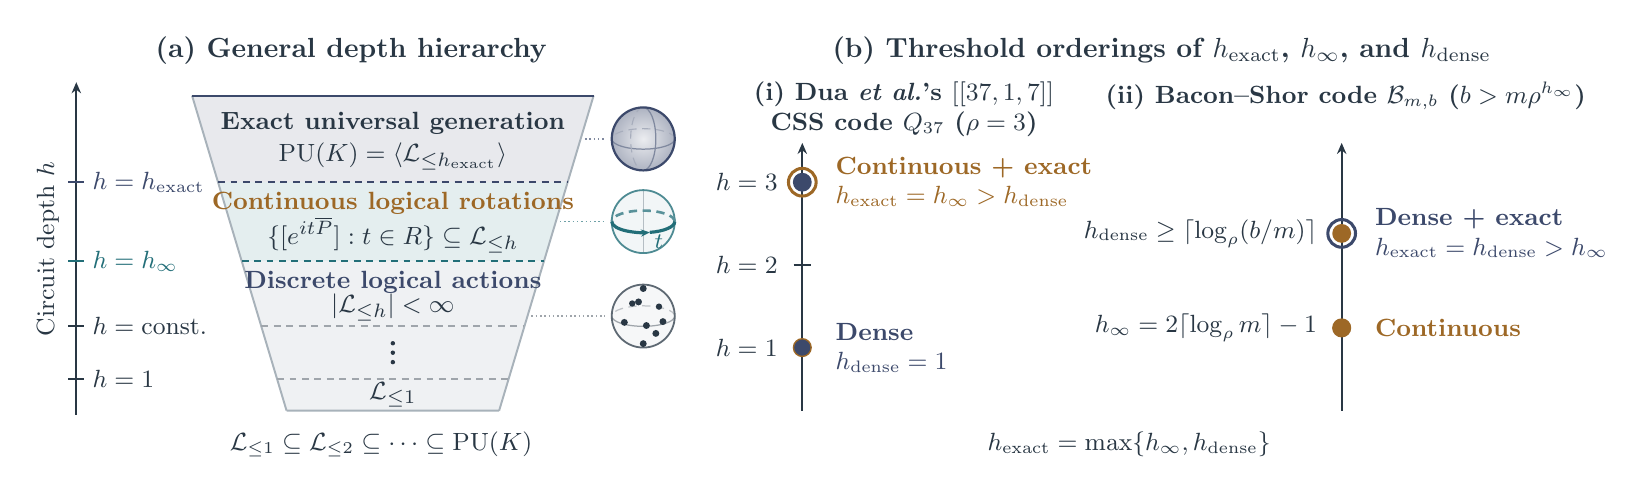
\begin{tikzpicture}[
  x=1cm,y=1cm,font=\rmfamily\fontsize{9.5}{11}\selectfont,text=FOneInk,
  f2panel/.style={anchor=center,font=\rmfamily\bfseries\fontsize{10}{11.5}\selectfont,text=FOneInk},
  f2sub/.style={anchor=north,align=center,font=\rmfamily\bfseries\fontsize{9}{10.8}\selectfont,text=FOneInk},
  f2head/.style={font=\rmfamily\bfseries\fontsize{9}{10.5}\selectfont},
  f2tick/.style={font=\rmfamily\fontsize{9}{10.5}\selectfont,anchor=west,inner sep=0pt},
  f2cap/.style={dash pattern=on 2.5pt off 2pt,line width=0.7pt},
  f2axis/.style={draw=FOneInk,line width=0.65pt,-{Stealth[length=4pt,width=3.4pt]}}
]
% ============================================================
% Panel (a): General depth hierarchy + Bloch-sphere schematics
% ============================================================
\begin{scope}[local bounding box=f2hierarchy]

% Upward depth axis
\draw[f2axis] (0.48,0.50)--(0.48,4.72);
\node[rotate=90] at (0.12,2.60) {Circuit depth $h$};

% Trapezoid tiers (center x=4.50; bottom y=0.55, h_inf y=2.45, h_exact y=3.45, top y=4.55)
\path[fill=FOneWire!18]
  (3.15,0.55)--(5.85,0.55)--(6.42,2.45)--(2.58,2.45)--cycle;
\path[fill=FOneTeal!12]
  (2.58,2.45)--(6.42,2.45)--(6.72,3.45)--(2.28,3.45)--cycle;
\path[fill=FOneNavy!12]
  (2.28,3.45)--(6.72,3.45)--(7.05,4.55)--(1.95,4.55)--cycle;

% Trapezoid outer frame
\draw[FOneWire,line width=0.7pt]
  (3.15,0.55)--(1.95,4.55) (5.85,0.55)--(7.05,4.55) (3.15,0.55)--(5.85,0.55);
\draw[FOneNavy,line width=0.75pt] (1.95,4.55)--(7.05,4.55);

% Axis ticks and labels
\foreach \yy/\lab/\col in {
  0.95/1/FOneInk,
  1.62/\mathrm{const.}/FOneInk,
  2.45/h_\infty/FOneTeal,
  3.45/h_{\mathrm{exact}}/FOneNavy} {
  \draw[\col,line width=0.65pt] (0.38,\yy)--(0.58,\yy);
  \node[f2tick,text=\col] at (0.68,\yy) {$h=\lab$};
}

% Internal tier dividers and labels
\draw[FOneInk!45,f2cap] (3.03,0.95)--(5.97,0.95);
\draw[FOneInk!45,f2cap] (2.83,1.62)--(6.17,1.62);
\node at (4.50,0.75) {$\mathcal L_{\le 1}$};
\foreach \dy in {-0.12,0,0.12} {
  \fill[FOneInk] (4.50,{1.285+\dy}) circle[radius=0.8pt];
}
\node[f2head,text=FOneNavy] at (4.50,2.18) {Discrete logical actions};
\node at (4.50,1.86) {$\lvert\mathcal L_{\le h}\rvert<\infty$};

% Continuous tier
\draw[FOneTeal,f2cap] (2.58,2.45)--(6.42,2.45);
\node[f2head,text=FOneAmber] at (4.50,3.18) {Continuous logical rotations};
\node at (4.50,2.78) {$\{[e^{it\overline P}]:t\in\mathbb R\}\subseteq\mathcal L_{\le h}$};

% Exact universal tier
\draw[FOneNavy,f2cap] (2.28,3.45)--(6.72,3.45);
\node[f2head] at (4.50,4.20) {Exact universal generation};
\node at (4.50,3.78) {$\PU(K)=\langle\mathcal L_{\le h_{\mathrm{exact}}}\rangle$};

\node[anchor=center,font=\rmfamily\fontsize{8.8}{10}\selectfont] at (4.35,0.12)
  {$\mathcal L_{\le 1}\subseteq\mathcal L_{\le 2}\subseteq\cdots\subseteq\PU(K)$};

% --- Three Bloch spheres aligned with the three tiers (centered at x=7.68, R=0.40) ---
% Subtle dotted connectors from trapezoid right edge to each sphere
\draw[FOneInk!45,densely dotted,line width=0.55pt] (6.26,1.75)--(7.20,1.75);
\draw[FOneTeal!65,densely dotted,line width=0.55pt] (6.62,2.95)--(7.20,2.95);
\draw[FOneNavy!65,densely dotted,line width=0.55pt] (6.94,4.00)--(7.20,4.00);

% 1. Bottom sphere: Discrete points
\begin{scope}[shift={(7.68,1.75)}]
  \fill[FOneWire!10] (0,0) circle[radius=0.40];
  \draw[FOneInk!30,densely dashed,line width=0.45pt]
    (0.40,0) arc[start angle=0,end angle=180,x radius=0.40,y radius=0.13];
  \draw[FOneInk!45,line width=0.45pt]
    (-0.40,0) arc[start angle=180,end angle=360,x radius=0.40,y radius=0.13];
  \draw[FOneInk!75,line width=0.65pt] (0,0) circle[radius=0.40];
  % Back-hemisphere discrete points
  \foreach \px/\py in {-0.14/0.16, 0.20/0.12} {
    \fill[FOneInk] (\px,\py) circle[radius=1.15pt];
  }
  % Front-hemisphere discrete points
  \foreach \px/\py in {0.00/0.35, 0.00/-0.35, -0.24/-0.08, 0.04/-0.12, 0.25/-0.07, -0.06/0.18, 0.16/-0.22} {
    \fill[FOneInk] (\px,\py) circle[radius=1.25pt];
  }
\end{scope}

% 2. Middle sphere: 1-parameter continuous curve (t)
\begin{scope}[shift={(7.68,2.95)}]
  \fill[FOneTeal!6] (0,0) circle[radius=0.40];
  % Faint vertical rotation axis
  \draw[FOneWire!85,line width=0.45pt] (0,-0.40)--(0,0.40);
  \draw[FOneTeal!80,line width=0.65pt] (0,0) circle[radius=0.40];
  % Continuous 1-parameter orbit (back dashed, front solid with arrow)
  \draw[FOneTeal!75,densely dashed,line width=0.95pt]
    (0.40,0) arc[start angle=0,end angle=180,x radius=0.40,y radius=0.14];
  \draw[FOneTeal,line width=1.15pt,-{Stealth[length=3.2pt,width=2.6pt]}]
    (-0.40,0) arc[start angle=180,end angle=282,x radius=0.40,y radius=0.14];
  \draw[FOneTeal,line width=1.15pt]
    (0.083,-0.137) arc[start angle=282,end angle=360,x radius=0.40,y radius=0.14];
  \node[text=FOneTeal,font=\rmfamily\fontsize{8.2}{9}\selectfont] at (0.20,-0.25) {$t$};
\end{scope}

% 3. Top sphere: Full surface covered (PU(K))
\begin{scope}[shift={(7.68,4.00)}]
  \shade[inner color=FOneNavy!10,outer color=FOneNavy!42] (0,0) circle[radius=0.40];
  % Subtle latitude and meridian lines to convey full 2D surface coverage
  \draw[FOneNavy!45,densely dashed,line width=0.4pt]
    (0.40,0) arc[start angle=0,end angle=180,x radius=0.40,y radius=0.13];
  \draw[FOneNavy!65,line width=0.45pt]
    (-0.40,0) arc[start angle=180,end angle=360,x radius=0.40,y radius=0.13];
  \draw[FOneNavy!45,densely dashed,line width=0.4pt]
    (0,0.40) arc[start angle=90,end angle=270,x radius=0.16,y radius=0.40];
  \draw[FOneNavy!65,line width=0.45pt]
    (0,-0.40) arc[start angle=-90,end angle=90,x radius=0.16,y radius=0.40];
  \draw[FOneNavy,line width=0.8pt] (0,0) circle[radius=0.40];
\end{scope}
\end{scope}
\node[f2panel] at (f2hierarchy.center |- 0,5.12) {(a) General depth hierarchy};

% ============================================================
% Panel (b): Threshold orderings (vertical)
% ============================================================
\begin{scope}[local bounding box=f2orderings]

% --- Track (i): Dua et al.'s [[37,1,7]] CSS code Q_37 ---
\begin{scope}[local bounding box=f2dua]

% Upward axis & ticks
\draw[f2axis] (9.70,0.55)--(9.70,3.95);
\foreach \yy/\n in {1.35/1, 2.40/2, 3.45/3} {
  \draw[FOneInk,line width=0.6pt] (9.59,\yy)--(9.81,\yy);
  \node[anchor=east,font=\rmfamily\fontsize{9}{10.5}\selectfont] at (9.51,\yy) {$h=\n$};
}

% Event markers and labels for Q_37
\fill[FOneNavy] (9.70,1.35) circle[radius=3.2pt];
\draw[FOneAmber,line width=0.5pt] (9.70,1.35) circle[radius=3.2pt];
\node[anchor=west,align=left,text=FOneNavy,font=\rmfamily\fontsize{8.8}{10.5}\selectfont]
  at (10.00,1.35) {\textbf{Dense}\\$h_{\mathrm{dense}}=1$};

\fill[FOneNavy] (9.70,3.45) circle[radius=3.4pt];
\draw[FOneAmber,line width=1.1pt] (9.70,3.45) circle[radius=5.0pt];
\node[anchor=west,align=left,text=FOneAmber,font=\rmfamily\fontsize{8.8}{10.5}\selectfont]
  at (10.00,3.45) {\textbf{Continuous + exact}\\$h_{\mathrm{exact}}=h_\infty>h_{\mathrm{dense}}$};
\end{scope}
\node[f2sub] at (f2dua.center |- 0,4.85)
  {(i) Dua \emph{et al.}'s $[[37,1,7]]$\\ CSS code $Q_{37}$ ($\rho=3$)};

% --- Track (ii): Elongated Bacon-Shor code B_{m,b} ---
\begin{scope}[local bounding box=f2baconshor]

% Upward axis & ticks
\draw[f2axis] (16.55,0.55)--(16.55,3.95);
\draw[FOneTeal,line width=0.65pt] (16.44,1.60)--(16.66,1.60);
\node[anchor=east,text=FOneInk,font=\rmfamily\fontsize{9}{10.5}\selectfont]
  at (16.36,1.60) {$h_\infty=2\lceil\log_\rho m\rceil-1$};
\draw[FOneNavy,line width=0.65pt] (16.44,2.80)--(16.66,2.80);
\node[anchor=east,text=FOneInk,font=\rmfamily\fontsize{9}{10.5}\selectfont]
  at (16.36,2.80) {$h_{\mathrm{dense}}\ge\lceil\log_\rho(b/m)\rceil$};

% Event markers and labels for Bacon-Shor
\fill[FOneAmber] (16.55,1.60) circle[radius=3.2pt];
\draw[FOneAmber,line width=0.5pt] (16.55,1.60) circle[radius=3.2pt];
\node[anchor=west,align=left,text=FOneAmber,font=\rmfamily\fontsize{8.8}{10.5}\selectfont]
  at (16.85,1.60) {\textbf{Continuous}};

\fill[FOneAmber] (16.55,2.80) circle[radius=3.4pt];
\draw[FOneNavy,line width=1.1pt] (16.55,2.80) circle[radius=5.0pt];
\node[anchor=west,align=left,text=FOneNavy,font=\rmfamily\fontsize{8.8}{10.5}\selectfont]
  at (16.85,2.80) {\textbf{Dense + exact}\\$h_{\mathrm{exact}}=h_{\mathrm{dense}}>h_\infty$};
\end{scope}
\node[f2sub] at (f2baconshor.center |- 0,4.85)
  {(ii) Bacon--Shor code $\mathcal B_{m,b}$ ($b>m\rho^{h_\infty}$)};

% Bottom summary for panel (b)
\node[anchor=center,font=\rmfamily\fontsize{8.8}{10}\selectfont,text=FOneInk]
  at (13.85,0.12) {$h_{\mathrm{exact}}=\max\{h_\infty,h_{\mathrm{dense}}\}$};
\end{scope}
\node[f2panel] at (f2orderings.center |- 0,5.12)
  {(b) Threshold orderings of $h_{\mathrm{exact}}$, $h_\infty$, and $h_{\mathrm{dense}}$};
\end{tikzpicture}%
}
\caption{\rev{Depth hierarchy of exact logical symmetries and threshold orderings.
(a) General hierarchy: the allowed logical images grow by inclusion, remaining finite below
$h_\infty$; for qubit stabilizer codes, continuous rotations emerge at
$h_\infty=2\lceil\log_\rho d\rceil-1$, and exact universal generation by finite words begins at
$h_{\mathrm{exact}}=\max\{h_\infty,h_{\mathrm{dense}}\}$.
(b) Concrete examples showing that continuous control ($h_\infty$) and dense generation
($h_{\mathrm{dense}}$) can occur in either order: (i) for Dua \emph{et al.}'s $[[37,1,7]]$ CSS
code $Q_{37}$ at $\rho=3$, dense generation appears first at $h_{\mathrm{dense}}=1$ while
continuous rotations and exact generation appear together at $h_{\mathrm{exact}}=h_\infty=3$
(exact integer depths); (ii) for elongated Bacon--Shor subsystem codes $\mathcal B_{m,b}$ with
$b>m\rho^{h_\infty}$, continuous rotations about the short axis appear first at
$h_\infty=2\lceil\log_\rho m\rceil-1$, followed by dense and exact generation at
$h_{\mathrm{exact}}=h_{\mathrm{dense}}\ge\lceil\log_\rho(b/m)\rceil>h_\infty$ (schematic vertical
positions). In both examples, $h$ bounds the depth of each generator in a finite word rather than
the total synthesis depth.}}
\label{fig:logical-hierarchy}
\end{figure*}

\rev{The minima are over positive integers, with value $\infty$ for an empty defining set; the closure
is taken in the usual Lie group topology. Circuit reversal makes $\mathcal L_{\le h}$
closed under inversion, so the generated group consists of finite words in its elements. The first
threshold concerns one bounded-depth logical image. The second and third concern approximation
and exact synthesis by finite words, respectively: the depth bound applies to each generator, and
a word of $r$ generators has physical depth at most $rh$, with no prescribed bound on $r$.}

\rev{Exact generation requires dense generation and an infinite logical image, since a finite
alphabet generates only countably many words while $\PU(K)$ is uncountable. Thus
$h_{\mathrm{exact}}\ge\max\{h_\infty,h_{\mathrm{dense}}\}$. When
Eq.~\eqref{eq:correctable} holds for $d\ge2$, Theorem~\ref{thm:depth} further gives}

\begin{equation}\label{eq:critical-lower}
 h_{\mathrm{exact}}\ge h_\infty
 \ge2\lceil\log_\rho d\rceil-1.
\end{equation}

\rev{Neither condition alone is sufficient: a finite alphabet may generate densely, while a
continuous family may only rotate about one logical axis. Even infinitude and dense generation
together do not suffice for arbitrary sets, since a countable dense subgroup still has only
countably many finite words. The circuit model supplies additional regularity: its logical image at fixed depth is semialgebraic. An infinite such image contains a nonconstant smooth curve, and
density lets conjugates of its tangent span every logical direction. Theorem~\ref{thm:thresholds}
shows that this suffices for exact generation and also determines $h_\infty$ for every qubit
stabilizer code (Fig.~\ref{fig:logical-hierarchy}).}

\begin{theorem}\label{thm:thresholds}
\rev{Let $n\ge1$ and $\rho\ge2$ be integers. Consider $n$ physical subsystems of finite dimension
and arbitrary native unitary gates acting on at most $\rho$ of them.}
\begin{enumerate}
\item[(1)] For every $[[n,k,d]]$ qubit stabilizer code  $\mathcal C$ with $k\ge1$ and
actual distance $d\ge2$, the lower bound in Eq.~\eqref{eq:critical-lower} is tight:
\begin{equation}\label{eq:critical}
 h_\infty(\mathcal C,\rho)=2\lceil\log_\rho d\rceil-1,
\end{equation}
and $\mathcal L_{\le h_\infty}(\mathcal C,\rho)$ contains a nontrivial one-parameter subgroup.
\item[(2)] For every finite-dimensional quantum subsystem code $\mathcal C$ ($\dim\HH_L\ge2$,
$\dim\HH_G\ge1$) under Eq.~\eqref{eq:encoded},
\begin{equation}\label{eq:exact-max}
 h_{\mathrm{exact}}(\mathcal C,\rho)
 =\max\{h_\infty(\mathcal C,\rho),\,h_{\mathrm{dense}}(\mathcal C,\rho)\}.
\end{equation}
\end{enumerate}
\end{theorem}

\begin{proof}[Proof of part (1)]
Equation~\eqref{eq:critical-lower} gives $h_\infty\ge2\lceil\log_\rho d\rceil-1$. Conversely, a
stabilizer code of actual distance $d$ has a Hermitian logical Pauli $P$ of weight $d$ with
nonscalar logical action $\overline P$~\cite[Sec.~3.2]{GottesmanStabilizer}.

For any Hermitian Pauli of weight $w\ge2$, partition its active factors in each layer into disjoint
groups of size $\rho$ and at most one smaller group. A Clifford gate on each group concentrates its
Pauli product onto one representative~\cite{BonetMonroig,Cowtan,HaahLiuTan}. After $j$ rounds the
active weight is $\lceil w/\rho^j\rceil$. With $r=\lceil\log_\rho w\rceil$, $r-1$ rounds yield a
circuit $C$ such that $Q=CPC^\dagger$ is supported on at most $\rho$ sites, so
\begin{equation}\label{eq:pauli-family}
 U(t)=C^\dagger e^{itQ}C=e^{itP}
\end{equation}
has depth at most $2r-1$ for every $t\in\mathbb R$. Applying this to the weight-$d$ logical Pauli
implements the nontrivial one-parameter subgroup $[e^{it\overline P}]$ exactly on the subspace
code, giving $h_\infty\le 2\lceil\log_\rho d\rceil-1$.
\end{proof}


\begin{figure}[t]
\centering
\resizebox{\linewidth}{!}{%
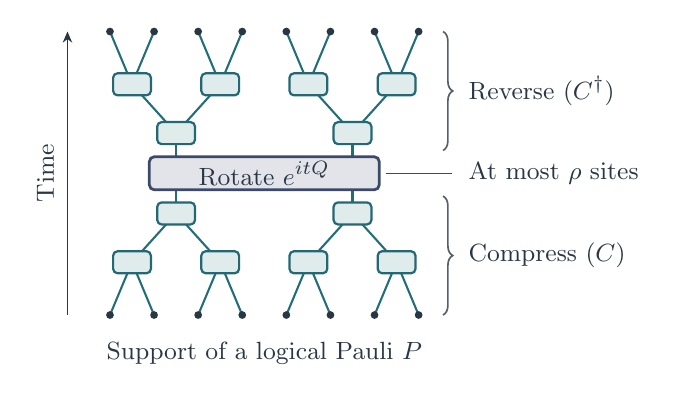
\begin{tikzpicture}[
  x=1cm,y=1cm,font=\rmfamily\fontsize{9.5}{11}\selectfont,text=FOneInk,
  f1tree/.style={draw=FOneTeal,line width=0.75pt},
  f1cliff/.style={draw=FOneTeal!90!FOneInk,fill=FOneTeal!14,line width=0.8pt,
    rounded corners=1.6pt,minimum width=0.48cm,minimum height=0.28cm,inner sep=0pt},
  f1brace/.style={draw=FOneInk!80,line width=0.6pt,
    decorate,decoration={brace,amplitude=3.5pt}}
]
% Time axis
\draw[FOneInk,line width=0.6pt,-{Stealth[length=4pt,width=3.4pt]}]
  (0.36,0.65)--(0.36,4.25);
\node[rotate=90] at (0.08,2.45) {Time};

% Active Pauli support tree lines
\foreach \a/\b/\c in {0.90/1.46/1.18, 2.02/2.58/2.30, 3.14/3.70/3.42, 4.26/4.82/4.54} {
  \draw[f1tree] (\a,0.65)--(\c,1.32)--(\b,0.65);
  \draw[f1tree] (\a,4.25)--(\c,3.58)--(\b,4.25);
  \fill[FOneInk] (\a,0.65) circle[radius=1.4pt];
  \fill[FOneInk] (\b,0.65) circle[radius=1.4pt];
  \fill[FOneInk] (\a,4.25) circle[radius=1.4pt];
  \fill[FOneInk] (\b,4.25) circle[radius=1.4pt];
}
\foreach \a/\b/\c in {1.18/2.30/1.74, 3.42/4.54/3.98} {
  \draw[f1tree] (\a,1.32)--(\c,1.94)--(\b,1.32);
  \draw[f1tree] (\a,3.58)--(\c,2.96)--(\b,3.58);
  \draw[f1tree] (\c,1.94)--(\c,2.24);
  \draw[f1tree] (\c,2.96)--(\c,2.66);
}

% Clifford compression gates
\foreach \c in {1.18,2.30,3.42,4.54} {
  \node[f1cliff] at (\c,1.32) {};
  \node[f1cliff] at (\c,3.58) {};
}
\foreach \c in {1.74,3.98} {
  \node[f1cliff] at (\c,1.94) {};
  \node[f1cliff] at (\c,2.96) {};
}

% Central rotation layer
\draw[draw=FOneNavy,fill=FOneNavy!15,line width=1.0pt,rounded corners=1.8pt]
  (1.40,2.24) rectangle (4.32,2.66);
\node[text=FOneInk] at (2.86,2.45) {Rotate $e^{itQ}$};

% Right-side braces and annotations
\draw[f1brace] (5.13,4.25)--(5.13,2.74);
\node[anchor=west] at (5.33,3.495) {Reverse ($C^\dagger$)};
\draw[FOneNavy,line width=0.55pt] (4.40,2.45)--(5.25,2.45);
\node[anchor=west] at (5.33,2.45) {At most $\rho$ sites};
\draw[f1brace] (5.13,2.16)--(5.13,0.65);
\node[anchor=west] at (5.33,1.405) {Compress ($C$)};

\node[anchor=center] at (2.86,0.16) {Support of a logical Pauli $P$};
\end{tikzpicture}%
}
\caption{\rev{Continuous logical rotation at the critical depth $2\lceil\log_\rho d\rceil-1$ (time runs upward).
A Clifford compression tree $C$ of $\lceil\log_\rho d\rceil-1$ layers concentrates a weight-$d$
logical Pauli $P$ onto $Q=CPC^\dagger$ supported on at most $\rho$ sites, followed by a
single-layer rotation $e^{itQ}$ and the reversal $C^\dagger$, implementing the continuous
subgroup $e^{it\overline P}$.}}
\label{fig:mechanisms}
\end{figure}

\begin{proof}[Proof of part (2)]
As noted before Eq.~\eqref{eq:critical-lower},
$h_{\mathrm{exact}}\ge\max\{h_\infty,h_{\mathrm{dense}}\}$ (including when either threshold is
$\infty$). \rev{For the converse}, \rev{we combine semialgebraicity with the Lie group mechanism
used in exact universality arguments~\cite{HarrowExact}. Fix} a finite depth
$h\ge\max\{h_\infty,h_{\mathrm{dense}}\}$, so $\mathcal
L_{\le h}(\mathcal C,\rho)$ is infinite and $G=\langle\mathcal L_{\le h}(\mathcal C,\rho)\rangle$
is dense in $\PU(K)$. For each support arrangement $\alpha$, unitarity and Eq.~\eqref{eq:encoded}
define a compact real algebraic set in the real and imaginary entries of the local gates, $W$, and
$Z$. Projecting onto the real conjugation coordinates of $X\mapsto WXW^\dagger$ and taking the
finite union over $\alpha$ makes $\mathcal L_{\le h}(\mathcal C,\rho)$ a compact real semialgebraic
set~\cite{BasuPollackRoy}.

Because $\mathcal L_{\le h}(\mathcal C,\rho)$ is infinite, a positive-dimensional smooth
semialgebraic stratum contains a smooth curve $a(t)$ near $0$ with $a'(0)\ne0$. By inverse-closure,
$c(t)=a(t)a(0)^{-1}$ lies in $G$ with $c(0)=e$ and nonzero tangent $X=c'(0)\in\mathfrak{su}(K)$.
The $\operatorname{Ad}_G$-invariant subspace $E=\operatorname{span}_{\mathbb
R}\{\operatorname{Ad}_g X:g\in G\}$ is finite-dimensional, hence closed, so density of $G$ makes
$E$ $\operatorname{Ad}_{\PU(K)}$-invariant---a nonzero ideal of the simple real Lie algebra
$\mathfrak{su}(K)$---forcing $E=\mathfrak{su}(K)$. Choosing $g_1,\ldots,g_N\in G$ ($N=K^2-1$) so
that $\{\operatorname{Ad}_{g_j}X\}$ is a basis of $\mathfrak{su}(K)$, the product map
$(t_1,\ldots,t_N)\mapsto\prod_{j=1}^N g_jc(t_j)g_j^{-1}$ has invertible derivative at the origin.
By the inverse function theorem, $G$ contains an identity neighborhood in $\PU(K)$ and is thus an
open subgroup of the connected group $\PU(K)$, giving $G=\PU(K)$ and $h_{\mathrm{exact}}\le h$.
\end{proof}

\rev{The thresholds $h_\infty$ and $h_{\mathrm{dense}}$ can occur in either order. For the
$[[37,1,7]]$ CSS code $Q_{37}$ of Dua \emph{et al.}~\cite{Dua}, take $\rho=3$. Two depth-one gate
partitions implement $\overline T^\dagger$ and $\sqrt{\overline X}^{\,\dagger}$. Their finite
words include $\overline H$ and $\overline T$, which generate a dense subgroup of
$\PU(2)$~\cite{Boykin}. Thus $h_{\mathrm{dense}}=1$, although the logical images at depths one and two are finite. Theorem~\ref{thm:thresholds} gives
$h_\infty=h_{\mathrm{exact}}=3$: approximate universality precedes continuous logical control.
An explicit depth-three rotation is given in the Supplemental Material~\cite{Supplement}.}

Rectangular Bacon--Shor subsystem codes \rev{give} the \rev{reverse} ordering~\cite{Supplement}. On an
$m\times b$ rectangle, $2\le m\le b$, \rev{a} bare logical $\overline X$ has a column representative
$P_X$ of weight $m$\rev{, while the} other bare axes have weight at least $b$\rev{. The short axis gives
$h_\infty=2\lceil\log_\rho m\rceil-1$}. If $m\rho^h<b$, the normalized gauge trace of the code
compression of $UP_XU^\dagger$ lies in
$\operatorname{span}_{\mathbb C}\{\id_L,\overline X\}$ for every \rev{allowed} circuit of depth $h$.
Hence $W\overline XW^\dagger=\pm\overline X$, \rev{so} the generated group and its closure preserve
\rev{this} axis. Taking $b>m\rho^{h_\infty}$ gives \rev{$h_\infty<h_{\mathrm{dense}}=h_{\mathrm{exact}}$}.
\rev{Here continuous control is available before} the \rev{logical directions needed} for \rev{universality can
be generated}.


\section*{\rev{Fault suppression at different depths}}
\rev{The light cone geometry that constrains logical
actions also governs fault recovery. We ask how much suppression code distance guarantees over
all exact circuits within a given depth budget.}

\rev{Consider an exact code-preserving circuit of depth at most $h$, with gates on at most $\rho$
original qubits of a stabilizer code $\mathcal C$. We encode the input ideally and apply an optimal ideal recovery only at the output. Each gate location independently fails with
probability $p$, applying a nonidentity Pauli on its support; every such Pauli has positive
conditional probability independent of $p$. Let $\epsilon_{\rm L}^{\rm opt}(p)$ be the minimum
logical entanglement infidelity over terminal recovery channels. It equals the optimal logical
Pauli failure probability when the effective physical noise is Pauli; the definition also applies
to arbitrary native unitaries (Supplemental Material, Eqs.~\eqref{eq:logical-entanglement-infidelity}
and~\eqref{eq:optimal-pauli-decoding}).}

\rev{For a fixed code and circuit, the suppression exponent is the largest integer $m$ (or $\infty$)
such that $\epsilon_{\rm L}^{\rm opt}(p)=O(p^m)$ as $p\to0$. Its minimum over all admissible
circuits of depth at most $h$ is $m_{\rm pc}(\mathcal C;\rho,h)$. A lower bound on $m_{\rm pc}$
therefore applies to every allowed implementation, while an upper bound identifies a circuit on that code with the corresponding vulnerability. We establish two universal envelopes for codes of actual distance
$d$:}

\begin{revision}\begin{equation}\label{eq:envelopes-def}
 m_-(h)=\left\lceil\frac{d}{\rho^h+\rho}\right\rceil,
 \qquad
 m_+(h)=\left\lceil\frac{d}{2\rho^{\lceil h/2\rceil}}\right\rceil .
\end{equation}\end{revision}

\rev{Every such code obeys $m_-(h)\le m_{\rm pc}\le m_+(h)$. For the lower bound, consider a cross
term between two histories containing at most $r$ faults each. A fault in layer $\ell$ has input
and output light cones of sizes at most $\rho^\ell$ and $\rho^{h-\ell+1}$. Since their sum is at
most $\rho^h+\rho$, the cross term acts on at most $r(\rho^h+\rho)$ qubits in at least one frame.
If this is less than $d$, error detection and exact code preservation make its code compression
scalar. The Knill--Laflamme conditions hold jointly for all histories with fewer than $m_-(h)$
faults~\cite{KL}. For $N_{\rm loc}$ locations, this gives, even under local stochastic Pauli noise
of strength $p$,}

\begin{equation}\label{eq:discussion-noise-exponent}
 \epsilon_{\rm L}^{\rm opt}(p)
 \le \binom{N_{\rm loc}}{m_-(h)}\,p^{m_-(h)}.
\end{equation}

\rev{The upper bound follows by compressing blocks of a minimum-weight logical Pauli, inserting
faults near the circuit midpoint, and undoing the compression. Two histories with at most
$m_+(h)$ faults each then produce errors differing by that logical Pauli, which no common terminal
recovery can correct simultaneously.}

\begin{figure}[htbp]
\centering
\resizebox{\linewidth}{!}{%
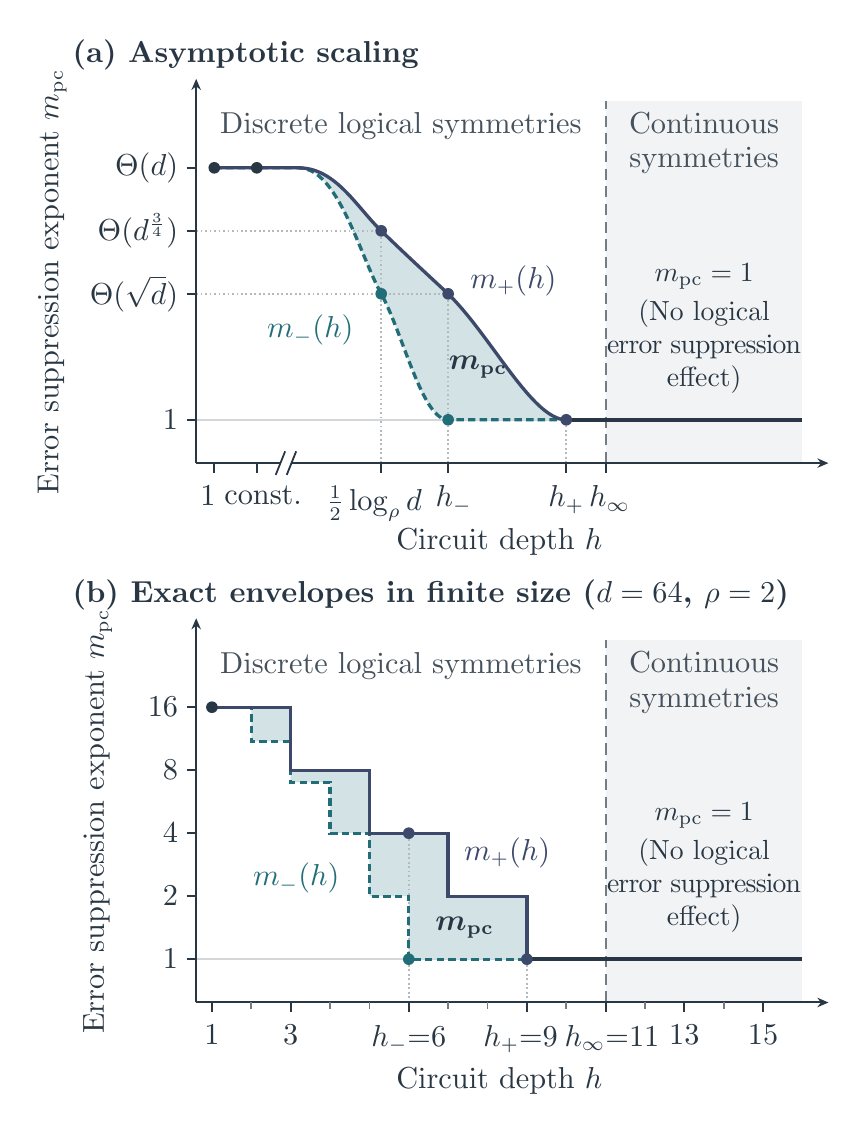
\begin{tikzpicture}[
  x=1cm,y=1cm,font=\rmfamily\fontsize{10.7}{12.5}\selectfont,text=FOneInk,
  inner sep=1.5pt,
  f3panel/.style={anchor=west,font=\rmfamily\bfseries\fontsize{11.1}{13}\selectfont},
  f3regime/.style={anchor=north,align=center,text=FOneInk!87},
  f3note/.style={align=center,font=\rmfamily\fontsize{10.35}{12}\selectfont},
  f3axis/.style={draw=FOneInk,line width=0.72pt,-{Stealth[length=4pt,width=3.4pt]}},
  f3tick/.style={draw=FOneInk,line width=0.65pt},
  f3minor/.style={f3tick,draw=FOneInk!65},
  f3guide/.style={draw=FOneInk!35,densely dotted,line width=0.62pt},
  f3threshold/.style={draw=FOneInk!65,dash pattern=on 4.0pt off 2.4pt,line width=0.72pt},
  f3upper/.style={draw=FOneNavy,line width=1.20pt},
  f3lower/.style={draw=FOneTeal,line width=1.20pt,dash pattern=on 2.7pt off 1.5pt},
  f3unity/.style={draw=FOneInk,line width=1.32pt}
]
\useasboundingbox (-0.99,-7.41) rectangle (9.31,6.33);
% ============================================================
% Panel (a): Qualitative asymptotic scaling (top)
% Plot box: x in [1.15, 8.85] (width 7.70), h_inf at x = 6.35
% ============================================================
\node[f3panel] at (-0.48,5.98) {(a) Asymptotic scaling};

% Regime background shading
\fill[white]   (1.15,0.80) rectangle (6.35,5.40);
\fill[FOneInk!6] (6.35,0.80) rectangle (8.85,5.40);
\draw[FOneInk!20,line width=0.62pt] (1.15,1.35)--(8.85,1.35);

% Shaded region between m_+(h) and m_-(h)
\path[fill=FOneTeal!20]
  (2.45,4.55)
  .. controls (2.92,4.55) and (3.18,4.06) .. (3.50,3.75)
  .. controls (3.82,3.44) and (4.06,3.22) .. (4.35,2.95)
  .. controls (4.90,2.41) and (5.42,1.35) .. (5.85,1.35)
  -- (4.35,1.35)
  .. controls (4.02,1.35) and (3.78,2.44) .. (3.50,2.95)
  .. controls (3.22,3.46) and (2.95,4.55) .. (2.45,4.55)
  -- cycle;

% Dotted reference guides
\draw[f3guide] (1.15,3.75)--(3.50,3.75) (3.50,0.80)--(3.50,3.75);
\draw[f3guide] (1.15,2.95)--(4.35,2.95) (4.35,0.80)--(4.35,2.95);
\draw[f3guide] (5.85,0.80)--(5.85,1.35);
\draw[f3threshold] (6.35,0.80)--(6.35,5.40);

% Envelopes: m_+(h) solid navy, m_-(h) dashed teal, merged m=1 solid ink
\draw[f3lower]
  (1.38,4.55)--(2.45,4.55)
  .. controls (2.95,4.55) and (3.22,3.46) .. (3.50,2.95)
  .. controls (3.78,2.44) and (4.02,1.35) .. (4.35,1.35)
  --(5.85,1.35);
\draw[f3upper]
  (1.38,4.55)--(2.45,4.55)
  .. controls (2.92,4.55) and (3.18,4.06) .. (3.50,3.75)
  .. controls (3.82,3.44) and (4.06,3.22) .. (4.35,2.95)
  .. controls (4.90,2.41) and (5.42,1.35) .. (5.85,1.35);
\draw[f3unity] (5.85,1.35)--(8.85,1.35);

% Key point markers
\fill[FOneInk]  (1.38,4.55) circle[radius=2.1pt];
\fill[FOneInk]  (1.92,4.55) circle[radius=2.1pt];
\fill[FOneNavy] (3.50,3.75) circle[radius=2.1pt];
\fill[FOneTeal] (3.50,2.95) circle[radius=2.1pt];
\fill[FOneNavy] (4.35,2.95) circle[radius=2.1pt];
\fill[FOneTeal] (4.35,1.35) circle[radius=2.1pt];
\fill[FOneNavy] (5.85,1.35) circle[radius=2.1pt];

% Axes with scale break //
\draw[f3tick] (1.15,0.80)--(2.22,0.80);
\draw[f3tick] (2.16,0.65)--(2.28,0.95);
\draw[f3tick] (2.30,0.65)--(2.42,0.95);
\draw[f3axis] (2.36,0.80)--(9.18,0.80);
\draw[f3axis] (1.15,0.80)--(1.15,5.68);

% Axis labels
\node[rotate=90] at (-0.68,3.10)
  {Error suppression exponent $m_{\rm pc}$};
\node[anchor=center] at (5.00,-0.20)
  {Circuit depth $h$};

% Y-axis ticks
\foreach \yy/\lab in {
  4.55/$\Theta(d)$,
  3.75/$\Theta(d^{\frac34})$,
  2.95/$\Theta(\sqrt{d})$,
  1.35/$1$} {
  \draw[f3tick] (1.03,\yy)--(1.15,\yy);
  \node[anchor=east] at (0.98,\yy) {\lab};
}

% X-axis ticks
\foreach \tx/\lx/\lab in {
  1.38/1.30/$1$,
  1.92/2.00/const.,
  3.50/3.41/$\tfrac12\log_\rho d$,
  4.35/4.42/$h_-$,
  5.85/5.85/$h_+$,
  6.35/6.40/$h_\infty$} {
  \draw[f3tick] (\tx,0.68)--(\tx,0.80);
  \node[anchor=north] at (\lx,0.57) {\lab};
}

% Internal regime and curve labels
\node[f3regime] at (3.75,5.31) {Discrete logical symmetries};
\node[f3regime] at (7.60,5.31) {Continuous\\symmetries};
\node[text=FOneNavy] at (5.18,3.12) {$m_+(h)$};
\node[text=FOneTeal] at (2.60,2.49) {$m_-(h)$};
\node[font=\rmfamily\bfseries\fontsize{10.7}{12.5}\selectfont] at (4.73,2.02) {$\boldsymbol{m_{\rm pc}}$};
\node[f3note] at (7.60,2.51)
  {$m_{\rm pc}=1$\\[2pt](No logical\\\textls[-30]{error suppression}\\effect)};

% ============================================================
% Panel (b): Exact envelopes for d = 64, rho = 2 (bottom, aligned)
% Plot box: x in [1.15, 8.85] (width 7.70), h_inf = 11 at x = 6.35
% Mapping: x(h) = 1.35 + 0.50*(h - 1), y(m) = 1.35 + 0.80*log2(m)
% ============================================================
\begin{scope}[yshift=-6.85cm]
\node[f3panel] at (-0.48,5.98) {(b) Exact envelopes in finite size ($d=64$, $\rho=2$)};

% Regime background shading (h_inf = 11 at x = 6.35, aligned with panel a)
\fill[white]   (1.15,0.80) rectangle (6.35,5.40);
\fill[FOneInk!6] (6.35,0.80) rectangle (8.85,5.40);
\draw[FOneInk!20,line width=0.62pt] (1.15,1.35)--(8.85,1.35);

% Shaded region between exact upper and lower step envelopes
\path[fill=FOneTeal!20]
  (1.85,4.55)--(2.35,4.55)--(2.35,3.75)--(3.35,3.75)--(3.35,2.95)
  --(4.35,2.95)--(4.35,2.15)--(5.35,2.15)--(5.35,1.35)
  --(3.85,1.35)--(3.85,2.15)--(3.35,2.15)--(3.35,2.95)
  --(2.85,2.95)--(2.85,3.596)--(2.35,3.596)--(2.35,4.118)
  --(1.85,4.118)--cycle;

% Dotted reference guides at h_- = 6 (3.85), h_+ = 9 (5.35), h_inf = 11 (6.35)
\draw[f3guide] (3.85,0.80)--(3.85,2.95);
\draw[f3guide] (5.35,0.80)--(5.35,2.15);
\draw[f3threshold] (6.35,0.80)--(6.35,5.40);

% Exact step envelopes: m_+(h) solid navy, m_-(h) dashed teal, merged m=1 solid ink
\draw[f3lower]
  (1.35,4.55)--(1.85,4.55)--(1.85,4.118)--(2.35,4.118)--(2.35,3.596)
  --(2.85,3.596)--(2.85,2.95)--(3.35,2.95)--(3.35,2.15)
  --(3.85,2.15)--(3.85,1.35)--(5.35,1.35);
\draw[f3upper]
  (1.35,4.55)--(2.35,4.55)--(2.35,3.75)--(3.35,3.75)
  --(3.35,2.95)--(4.35,2.95)--(4.35,2.15)--(5.35,2.15)--(5.35,1.35);
\draw[f3unity] (5.35,1.35)--(8.85,1.35);

% Key point markers
\fill[FOneInk]  (1.35,4.55) circle[radius=2.1pt];
\fill[FOneNavy] (3.85,2.95) circle[radius=2.1pt];
\fill[FOneTeal] (3.85,1.35) circle[radius=2.1pt];
\fill[FOneNavy] (5.35,1.35) circle[radius=2.1pt];

% Axes
\draw[f3axis] (1.15,0.80)--(9.18,0.80);
\draw[f3axis] (1.15,0.80)--(1.15,5.68);

% Axis labels (aligned with panel a)
\node[rotate=90] at (-0.10,3.10)
  {Error suppression exponent $m_{\rm pc}$};
\node[anchor=center] at (5.00,-0.20)
  {Circuit depth $h$};

% Y-axis ticks (log2 scale aligned with panel a)
\foreach \yy/\lab in {4.55/16, 3.75/8, 2.95/4, 2.15/2, 1.35/1} {
  \draw[f3tick] (1.03,\yy)--(1.15,\yy);
  \node[anchor=east] at (0.98,\yy) {$\lab$};
}

% X-axis minor ticks for intermediate integers
\foreach \x in {1.85, 2.85, 3.35, 4.35, 4.85, 5.85, 6.85, 7.85} {
  \draw[f3minor] (\x,0.72)--(\x,0.80);
}
% X-axis major ticks with merged threshold labels
\foreach \tx/\lx/\lab in {
  1.35/1.35/$1$,
  2.35/2.35/$3$,
  3.85/3.85/$h_-{=}6$,
  5.35/5.27/$h_+{=}9$,
  6.35/6.43/$h_\infty{=}11$,
  7.35/7.35/$13$,
  8.35/8.35/$15$} {
  \draw[f3tick] (\tx,0.68)--(\tx,0.80);
  \node[anchor=north] at (\lx,0.57) {\lab};
}

% Internal regime and curve labels
\node[f3regime] at (3.75,5.31) {Discrete logical symmetries};
\node[f3regime] at (7.60,5.31) {Continuous\\symmetries};
\node[text=FOneNavy] at (5.10,2.70) {$m_+(h)$};
\node[text=FOneTeal] at (2.42,2.38) {$m_-(h)$};
\node[font=\rmfamily\bfseries\fontsize{10.7}{12.5}\selectfont] at (4.56,1.75) {$\boldsymbol{m_{\rm pc}}$};
\node[f3note] at (7.60,2.51)
  {$m_{\rm pc}=1$\\[2pt](No logical\\\textls[-30]{error suppression}\\effect)};
\end{scope}
\end{tikzpicture}%
}
\caption{Logical error suppression of the worst-case exponent $m_{\rm pc}$.
(a) Across constant depths, both envelopes $m_-(h)$ and $m_+(h)$
remain $\Theta(d)$. At logarithmic depths they separate, reaching $\Theta(\sqrt{d})$ versus
$\Theta_\rho(d^{3/4})$ at $h=\tfrac{1}{2}\log_\rho d$ and $1$ versus $\Theta(\sqrt{d})$ at
$h_-$. For $h\ge h_+$, $m_{\rm pc}=1$ ($\epsilon_{\rm L}^{\rm opt}=\Theta(p)$), where $h_+$ lies at most two layers below the continuous-symmetry threshold $h_\infty=2\lceil\log_\rho d\rceil-1$.
(b) Exact envelope values from Eq.~\eqref{eq:envelopes-def} for $\rho=2$ and $d=64$ on a
logarithmic vertical scale: $m_-(h)$ and $m_+(h)$ reach unity at $h_-=6$ and $h_+=9$,
respectively, while continuous logical control begins at $h_\infty=11$. Every stabilizer code of distance 64 has its worst-case exponent $m_{\rm pc}$ within the shaded band between the two
envelopes.}
\label{fig:depth-noise-symmetry}
\end{figure}

\rev{For $d>2\rho$, the envelopes first reach unity at}

\begin{equation}\label{eq:discussion-exponent-depths}
 h_- = \lceil\log_\rho(d-\rho)\rceil,\qquad
 h_+ = 2\lceil\log_\rho(d/2)\rceil-1.
\end{equation}

\rev{These depths satisfy $h_-\le h_+\le h_\infty$ and $h_\infty-h_+\in\{0,2\}$.
Below $h_-$, distance alone guarantees $m_{\rm pc}\ge2$. The Shor construction attains
$m_{\rm pc}=1$ at $h_-$, while the upper envelope remains greater than one until $h_+$.
For every $h\ge h_+$, each stabilizer code admits an implementation of depth at most $h$ with
$\epsilon_{\rm L}^{\rm opt}(p)=\Theta(p)$. Thus linear worst-case error can appear before
continuous logical control.}

\begin{theorem}[Sharp fault suppression bounds]\label{thm:fault-sharpness}
\rev{For every qubit stabilizer code $\mathcal C$ of actual distance $d\ge2$, and integers
$\rho\ge2$ and $h\ge1$, the independent Pauli noise model with optimal terminal recovery gives}
\begin{equation}\label{eq:discussion-fixed-code-exponent}
 \left\lceil\frac{d}{\rho^h+\rho}\right\rceil
 \le m_{\rm pc}(\mathcal C;\rho,h)
 \le \left\lceil\frac{d}{2\rho^{\lceil h/2\rceil}}\right\rceil.
\end{equation}
\rev{The bounds have the following saturation properties.}
\begin{enumerate}
\item[(1)] For every $d\ge2$, $\rho\ge2$, and $h\ge1$, there is an explicit stabilizer
code of actual distance $d$ with $m_{\rm pc}=m_-(h)$.
\item[(2)] For every fixed $\rho\ge2$ and all sufficiently large integers $t$, there is a high-rate
CSS subspace code $\mathcal C_t$ of length $\rho^{12t}$ and actual distance $d_t=\rho^{2t}$ with
$m_{\rm pc}(\mathcal C_t;\rho,h)=m_+(h)$ for $1\le h\le t$. At $h=t$, $m_+=\Theta_\rho(d_t^{3/4})$
strictly exceeds $m_-=\Theta(\sqrt{d_t})$.
\end{enumerate}
\rev{The bounds and both saturation} statements allow arbitrary native unitaries on the original
physical register.
\end{theorem}

\begin{proof}
The lower bound follows from Eq.~\eqref{eq:discussion-noise-exponent}. For the upper bound,
partition a weight-$d$ logical Pauli $P$ into $b=\lceil d/\rho^{\lceil h/2\rceil}\rceil$ blocks of
size at most $\rho^{\lceil h/2\rceil}$. For $h=2t$, compress each block to one site in $t$ layers,
absorb the resulting one-site Pauli into layer $t$ (applying a one-qubit Pauli gate if idle there),
and invert the compression in $t$ layers. For $h=2t+1$, compress each block to at most $\rho$ sites
in $t$ layers, apply its compressed Pauli as one middle gate, and invert. Both circuits implement
$P$ exactly, while a single midpoint fault in any block inserts that block's factor of $P$ at the
output.

Splitting these $b$ midpoint faults into two histories of sizes $\lfloor b/2\rfloor$ and $\lceil
b/2\rceil$ produces output errors with identical syndrome that differ by $P$. Under any common
terminal recovery, their conditional entanglement fidelities are overlaps of one recovered Choi
state with two orthogonal logical Choi vectors and thus sum to at most $1$. Since the less probable
history occurs with probability $\Theta(p^{\lceil b/2\rceil})$, $\epsilon_{\rm L}^{\rm
opt}(p)=\Omega(p^{\lceil b/2\rceil})$ even for $p$-dependent recovery, giving $m_{\rm pc}\le\lceil
b/2\rceil=m_+(h)$.

\rev{We prove both} saturation constructions in the Supplemental Material~\cite{Supplement}.
\end{proof}

\rev{In the Shor construction, a weight-$d$ row logical Pauli fixes the distance, while
equal-order fault histories near opposite ends of a logical identity circuit reach complementary
parts of a full-column logical Pauli. This attains $m_-(h)$ for every parameter triple.}

\rev{\emph{Shallow physical rigidity.}---The CSS construction also yields a structural result
independent of the noise model (Lemma S3 in the Supplemental Material~\cite{Supplement}). For the codes $\mathcal C_t$ in
Theorem~\ref{thm:fault-sharpness}, every exact code-preserving circuit of depth at most $t$ has a
total unitary equal, up to phase, to a product of single-qubit Paulis on the full physical Hilbert
space. This holds even when the native gates are arbitrary unitaries on at most $\rho$ of the
original qubits. Thus the result constrains the physical symmetries themselves, beyond their
induced logical actions. Support preservation under the total unitary then lets both light cone
bounds apply to each fault in the output frame, giving $m_{\rm pc}=m_+(h)$ for $1\le h\le t$.
At $h=t$, the attained exponents $\Theta(\sqrt d)$ and $\Theta_\rho(d^{3/4})$ show that the gap
between the envelopes reflects code structure.}

\section*{\rev{Discussion}}
\rev{Distance fixes the first continuous logical degree of freedom in a
stabilizer code, but it does not determine when the available gates generate every logical
direction or how well the code withstands its most damaging allowed circuit. The continuous control
and recovery bounds arise from the support reached by local perturbations, and $h_+$ and $h_\infty$ identify closely
spaced depths for linear worst-case error and continuous control. These are constraints on
logical accessibility and recovery guarantees over a circuit class. The suppression achievable
for a prescribed logical target, particularly with intermediate recovery, requires a separate
optimization.}

\textit{Acknowledgments.}--- We used generative AI tools for language editing and to assist with the
derivation and checking of the exact-generation results and the two examples. This work is
supported in part by the National Natural Science Foundation of China (NSFC) under Grant
No.~12475023, the Dushi Program, and startup funding from the Yau Mathematical Sciences Center
(YMSC).

\textit{Data availability.}---
Ref.~\cite{LeanRepo} provides Lean~4 formalizations of the statements of
Theorems~\ref{thm:depth}--\ref{thm:fault-sharpness}, including both saturation results,
and of the common error exponent for a fixed circuit. The audited declarations depend only on \texttt{propext},
\texttt{Classical.choice}, and \texttt{Quot.sound}.

\bibliography{depth}

\onecolumngrid
%\clearpage
\setcounter{equation}{0}
\renewcommand{\theequation}{S\arabic{equation}}
\renewcommand{\theHequation}{S\arabic{equation}}
\setcounter{lemma}{0}
\renewcommand{\thelemma}{S\arabic{lemma}}
\setcounter{proposition}{0}
\renewcommand{\theproposition}{S\arabic{proposition}}
\section*{Supplemental Material}

\rev{The \hyperref[sm:algebraic-finite-image]{algebraic finite-image criterion} gives the
\hyperref[sm:proof-thm-depth]{complete proof of Theorem~\ref*{thm:depth}}. We then specify the
\hyperref[sm:logical-error-measures]{terminal recovery model}, prove the two-frame recovery
bound, and establish the \hyperref[em:lower-saturation]{Shor lower saturation} and
\hyperref[em:upper-saturation]{CSS upper saturation}. The remaining sections give
\hyperref[sm:exact-synthesis]{constructive exact synthesis} and the two orderings of continuous
onset and dense generation in \hyperref[sm:bacon-shor]{Bacon--Shor codes} and the
\hyperref[sm:dua-example]{37-qubit CSS code}.}

\subsection*{Algebraic finite-image criterion}
\label{sm:algebraic-finite-image}

\rev{We use} the \rev{following finite-image} criterion in the proof of Theorem~\ref{thm:depth}. Let $r_1,\ldots,r_m$ be finitely many elements of a commutative coordinate
algebra $R$, representing the output coordinates of a polynomial map. An evaluation is a unital
$\mathbb C$-algebra homomorphism $\phi:R\to\mathbb C$. We seek to show that the set of output
tuples $(\phi(r_1),\ldots,\phi(r_m))$ is finite, without requiring either the set of evaluations or
the ambient parameter variety to be finite or smooth.

For each minimal prime ideal $\mathfrak p$ of $R$, set
\[
 F_{\mathfrak p}=\operatorname{Frac}(R/\mathfrak p),\qquad
 \iota_{\mathfrak p}:R\longrightarrow R/\mathfrak p
                         \longrightarrow F_{\mathfrak p}.
\]
Since $R/\mathfrak p$ is an integral domain, its canonical map into $F_{\mathfrak p}$ is injective
and $\ker\iota_{\mathfrak p}=\mathfrak p$. A $\mathbb C$-linear derivation $\delta:F_{\mathfrak
p}\to F_{\mathfrak p}$ is a $\mathbb C$-linear map obeying $\delta(xy)=\delta(x)y+x\delta(y)$.
\rev{The} derivations \rev{must be} tested in the function fields $F_{\mathfrak p}$ \rev{before specialization:}
every $\mathbb C$-linear derivation of $\mathbb C$ \rev{itself} vanishes.

\begin{lemma}\label{lem:algebraic-finite-image}
Let $R$ be a finitely generated commutative $\mathbb C$-algebra, and let $r_1,\ldots,r_m\in R$.
Suppose that, for every minimal prime $\mathfrak p$ of $R$ and every $\mathbb C$-linear derivation
$\delta:F_{\mathfrak p}\to F_{\mathfrak p}$,
\[
 \delta\bigl(\iota_{\mathfrak p}(r_i)\bigr)=0
 \quad\text{for every }i.
\]
Then the joint evaluation image
\[
 \{(\phi(r_1),\ldots,\phi(r_m)):
          \phi:R\to\mathbb C\text{ a }\mathbb C\text{-algebra map}\}
\]
is finite.
\end{lemma}

\begin{proof}
If $R=0$, no unital map $R\to\mathbb C$ exists and the image is empty. Assume $R\ne0$.

\emph{Constants in a function field.}---We first show that vanishing derivations force each output
coordinate to be constant on a component. Fix a minimal prime $\mathfrak p$ and write
$F=F_{\mathfrak p}$, which is finitely generated as a field over $\mathbb C$. Suppose $a\in F$ is
annihilated by every $\mathbb C$-linear derivation of $F$. If $a$ were transcendental over $\mathbb
C$, we could extend $\{a\}$ to a transcendence basis $B$ of $F/\mathbb C$ and take partial
differentiation $\partial$ with respect to $a$ on the rational function field $L=\mathbb C(B)$, so
that $\partial(a)=1$ while $B\setminus\{a\}$ and $\mathbb C$ are killed.

To obtain a contradiction, we extend this derivation from $L$ to $F$. Because $F/L$ is finitely
generated and algebraic in characteristic zero, it is finite and separable, so the primitive
element theorem gives $F=L(\beta)$ with minimal polynomial $f(T)=T^s+\sum_{j=0}^{s-1}a_jT^j\in
L[T]$. Differentiating $f(\beta)=0$ dictates
\[
 c=-\frac{\sum_{j=0}^{s-1}\partial(a_j)\beta^j}{f'(\beta)},
\]
where $f'(\beta)\ne 0$ by separability. For $g(T)=\sum_j b_jT^j\in L[T]$, define $D:L[T]\to F$ by
$D(g)=\sum_j\partial(b_j)\beta^j+g'(\beta)c$. This map satisfies $D(gh)=D(g)h(\beta)+g(\beta)D(h)$
and $D(f)=0$. It therefore descends through $L[T]/(f)\cong F$ to a $\mathbb C$-linear derivation of
$F$ extending $\partial$. The extension gives $D(a)=\partial(a)=1$, contradicting the assumption
that every such derivation annihilates $a$.

Hence $a$ is algebraic over $\mathbb C$, and thus $a\in\mathbb C$. Applying this to each
$\iota_{\mathfrak p}(r_i)$ yields constants $c_{i,\mathfrak p}\in\mathbb C$ such that
\begin{equation}\label{eq:component-constants}
 r_i-c_{i,\mathfrak p}\in\mathfrak p.
\end{equation}

\emph{From component constants to all evaluations.}---By Hilbert's basis theorem, $R$ is Noetherian
and therefore possesses a finite nonempty set of minimal primes $\{\mathfrak p_1,\ldots,\mathfrak
p_t\}$~\rev{\cite[Lemmas~10.31.6 and 10.17.2(3)]{Stacks}}. For any complex evaluation $\phi:R\to\mathbb C$, $\ker\phi$ is prime and thus
contains some minimal prime $\mathfrak p_\nu$~\rev{\cite[Lemma~10.17.2(4)]{Stacks}}. Applying $\phi$ to
Eq.~\eqref{eq:component-constants} gives $\phi(r_i)=c_{i,\mathfrak p_\nu}$ simultaneously for all
$i$ with the same index $\nu$, bounding the number of realized joint tuples by $t$.

\emph{Monic identities in the coordinate algebra.}---The same component constants also yield
identities within $R$, before evaluation. Forming $P_i(T)=\prod_{\nu=1}^{t}(T-c_{i,\mathfrak
p_\nu})$ gives $P_i(r_i)\in\bigcap_{\nu=1}^{t}\mathfrak p_\nu=\sqrt{(0)}$, the nilradical of
$R$~\rev{\cite[Lemma~10.17.2(4),(7)]{Stacks}}. Thus $P_i(r_i)^{a_i}=0$ for some integer $a_i\ge1$ (providing the monic
integrality polynomials used in the Lean formalization~\cite{LeanRepo}), which likewise forces
$P_i(\phi(r_i))=0$ at every complex evaluation $\phi$.
\end{proof}

Geometrically, the minimal primes represent the irreducible components of $\operatorname{Spec} R$.
Vanishing field derivations force the output map to be constant on each component, while nilpotent
directions (e.g., $r=\epsilon$ in $\mathbb C[t,\epsilon]/(\epsilon^2)$) evaluate to zero under
every homomorphism to $\mathbb C$. Consequently, neither reducedness, zero-dimensionality, nor
smoothness of physical evaluations is required. In Theorem~\ref{thm:depth}, $R=R_\alpha$ and the
conclusion holds directly at singular circuit configurations.

\subsection*{Complete proof of Theorem~\ref{thm:depth}}
\label{sm:proof-thm-depth}

\rev{The unitaries realizable at depth at most $h$ need not form a group, unlike fixed-partition
transversal gates~\cite{EK}. For each support arrangement, we express the circuit
and encoding constraints in a finitely generated coordinate algebra $R_\alpha$.
Lemma~\ref{lem:algebraic-finite-image} then gives a finite projective logical image without a
smoothness assumption on the associated complex variety.}

\begin{proof}[Proof of Theorem~\ref{thm:depth}]
\emph{Polynomial circuit constraints.}---We pad each circuit to $h$ layers and $n$ slots per layer
using identity gates on empty supports. \rev{Requiring} supports of size at most $\rho$, \rev{disjoint within each layer, leaves} finitely many
ordered support arrangements $\alpha$. Fix one arrangement
$\alpha$ and index its $J=nh$ slots in execution order. For slot $j$ with support $S_j$, take two
independent matrices on $\bigotimes_{i\in S_j}\HH_i$, extend both by the identity on the complement
to obtain $u_j,v_j$, and write $U=u_J\cdots u_1$. Take a $K\times K$ matrix $W$ and a $g\times g$
matrix $Z$, setting $Q=W\otimes Z$ as in Eq.~\eqref{eq:encoded}. The matrices $V$ and $V^\dagger$
have constant complex entries with $V^\dagger V=\id_L\otimes\id_G$.

Let $\mathbf x$ collect all matrix entries of the local factors of $u_j,v_j$ and of $W,Z$.
Introducing explicit inverse variables $v_j$ renders the circuit constraints purely polynomial.
Define $R_\alpha=\mathbb C[\mathbf x]/I_\alpha$, where $I_\alpha$ is generated by the entrywise
differences in
\begin{equation}
 u_jv_j=v_ju_j=\id,\quad UV=VQ,\quad V^\dagger U=QV^\dagger.\label{eq:algebraic-encoding}
\end{equation}
These constraints also make the logical and gauge factors invertible over $R_\alpha$. In
$R_\alpha$, $v_j=u_j^{-1}$ and $U^{-1}=v_1\cdots v_J$. The two encoding relations yield $(V^\dagger
U^{-1}V)Q=V^\dagger U^{-1}UV=\id_L\otimes\id_G$ and $Q(V^\dagger U^{-1}V)=V^\dagger
UU^{-1}V=\id_L\otimes\id_G$, so $Q^{-1}=V^\dagger U^{-1}V$ over $R_\alpha$.

Because $W\otimes\id_G$ and $\id_L\otimes Z$ commute and multiply to $Q$, their two-sided inverses
are $(\id_L\otimes Z)Q^{-1}$ and $(W\otimes\id_G)Q^{-1}$, respectively. Extracting a diagonal gauge
block of the inverse of $W\otimes\id_G$ gives $W^{-1}$. A diagonal logical block of the inverse of
$\id_L\otimes Z$ similarly gives $Z^{-1}$. Both inverses are thus matrices over $R_\alpha$.

Every physical circuit satisfying Eq.~\eqref{eq:encoded} induces a unital $\mathbb C$-algebra
evaluation $\phi:R_\alpha\to\mathbb C$ upon assigning $v_j=u_j^\dagger$. Indeed, $UV=VQ$ implies
$U^{-1}V=VQ^{-1}$, whose adjoint gives $V^\dagger U=QV^\dagger$ by unitarity of $U$ and $Q$.
General complex evaluations of $R_\alpha$ also include nonunitary solutions.

To record the logical action without its scalar phase, for $1\le a,b,c,e\le K$ define the $K^4$
conjugation coordinates in $R_\alpha$,
\begin{equation}\label{eq:conjugation-coordinates}
 r_{abce}=W_{ab}(W^{-1})_{ce},
\end{equation}
which record the matrix entries of $X\mapsto WXW^{-1}$ in the matrix-unit basis $\{\mathsf
e_{bc}\}$ via $W\mathsf e_{bc}W^{-1}=\sum_{a,e=1}^{K}r_{abce}\,\mathsf e_{ae}$.

\emph{Field derivations and error detection.}---To apply Lemma~\ref{lem:algebraic-finite-image}, we
must show that every field derivation annihilates these conjugation coordinates. Let $F/\mathbb C$
be an arbitrary field extension, $\phi:R_\alpha\to F$ a $\mathbb C$-algebra homomorphism, and
$\delta:F\to F$ a $\mathbb C$-linear derivation. In the following field argument, matrix symbols
denote their entrywise images under $\phi$. $\delta$ acts entrywise, and $V,V^\dagger$ remain
constant. Error detection extends linearly from $\mathbb C$ to $F$: any operator $O$ over $F$
supported on fewer than $d$ subsystems expands as $O=\sum_\mu a_\mu B_\mu$ with $a_\mu\in F$ and
complex matrix units $B_\mu$ satisfying Eq.~\eqref{eq:correctable}, giving $V^\dagger
OV=\id_L\otimes\sum_\mu a_\mu M_{B_\mu}$.

\emph{Two-frame support bounds.}---We now decompose the circuit variation into individual gate
insertions and bound each insertion from both ends of the circuit. Setting $U_{>j}=u_J\cdots
u_{j+1}$ and $U_{<j}=u_{j-1}\cdots u_1$ (empty products being $\id$), the Leibniz rule gives
$\delta(U)=\sum_{j=1}^J U_{>j}\delta(u_j)U_{<j}$. Multiplying on the right by
$U^{-1}=U_{<j}^{-1}u_j^{-1}U_{>j}^{-1}$ cancels $U_{<j}U_{<j}^{-1}$ in the $j$th term, yielding
\begin{equation}\label{eq:generator}
 \delta(U)U^{-1}=\sum_{j=1}^JU_{>j}\delta(u_j)u_j^{-1}U_{>j}^{-1}=\sum_{j=1}^J H_j=H.
\end{equation}
Transforming $H_j$ back to the input frame cancels $U_{>j}$ instead:
\[
 \begin{aligned}
 U^{-1}H_jU
 &=U_{<j}^{-1}u_j^{-1}\bigl(\delta(u_j)u_j^{-1}\bigr)u_jU_{<j}\\
 &=U_{<j}^{-1}u_j^{-1}\delta(u_j)U_{<j}.
 \end{aligned}
\]
Because the identity factors outside $S_j$ are constant, both $\delta(u_j)u_j^{-1}$ and
$u_j^{-1}\delta(u_j)$ are supported on $S_j$ and commute with all other disjoint gates in the same
layer. Conjugating an operator supported on a set $T$ by any single layer (or its inverse) spreads
its support only to the union of the disjoint gate blocks meeting $T$, enlarging the support size
by a factor of at most $\rho$.

For slot $j$ in layer $\ell\in\{1,\ldots,h\}$, the initial support $|S_j|\le\rho$
propagates through $h-\ell$ layers toward the output and $\ell-1$ layers toward the input, giving support bounds $\rho^{h-\ell+1}$ for $H_j$ and $\rho^\ell$ for $U^{-1}H_jU$. Since $\min\{h-\ell+1,\ell\}\le\lceil \frac{h}{2}\rceil$ and Eq.~\eqref{eq:depth} implies $h\le
2m-2$ for $m=\lceil\log_\rho d\rceil$, the smaller support satisfies $\rho^{\lceil
\frac{h}{2}\rceil}\le\rho^{m-1}<d$.

If $|\operatorname{supp}(H_j)|<d$, Eq.~\eqref{eq:correctable} directly gives $V^\dagger
H_jV=\id_L\otimes M_j$. Otherwise $|\operatorname{supp}(U^{-1}H_jU)|<d$, so input-frame detection
gives $V^\dagger U^{-1}H_jUV=\id_L\otimes N_j$. Using $V^\dagger U^{-1}=Q^{-1}V^\dagger$ and
$UV=VQ$, we transport this back to the output frame:
\begin{align*}
 V^\dagger H_jV &= Q(V^\dagger U^{-1}H_jUV)Q^{-1} \\
                &= Q(\id_L\otimes N_j)Q^{-1} = \id_L\otimes ZN_jZ^{-1}.
\end{align*}
In both cases $V^\dagger H_jV=\id_L\otimes M_j$, and summing over $j$ yields
\begin{equation}\label{eq:compression}
 V^\dagger HV=\id_L\otimes M,\qquad M=\sum_{j=1}^J M_j.
\end{equation}

\emph{From gauge-only compression to a finite logical image.}---The same compressed variation can
be computed from the encoded action. Differentiating $UV=VQ$ gives $\delta(U)V=V\delta(Q)$, which
together with $U^{-1}V=VQ^{-1}$ implies $V^\dagger HV=V^\dagger\delta(U)VQ^{-1}=\delta(Q)Q^{-1}$.
Expanding $Q=W\otimes Z$ gives
\begin{equation}\label{eq:logicalgen}
 \delta(Q)Q^{-1}
   =\delta(W)W^{-1}\otimes\id_G+\id_L\otimes\delta(Z)Z^{-1}.
\end{equation}
Equating this to $\id_L\otimes M$ from Eq.~\eqref{eq:compression} and extracting the $(1,1)$ gauge
block yields $\delta(W)W^{-1}=\lambda\id_L$ with $\lambda=(M-\delta(Z)Z^{-1})_{11}\in F$. Hence
$\delta(W)=\lambda W$ and $\delta(W^{-1})=-W^{-1}\delta(W)W^{-1}=-\lambda W^{-1}$, so every
conjugation coordinate satisfies
\[
 \delta\bigl(\phi(r_{abce})\bigr)
   =\lambda\phi(r_{abce})-\lambda\phi(r_{abce})=0.
\]
Specializing to $F=\operatorname{Frac}(R_\alpha/\mathfrak p)$ and the canonical map
$\phi=\iota_{\mathfrak p}$ for each minimal prime $\mathfrak p$ of $R_\alpha$ verifies the
hypothesis of Lemma~\ref{lem:algebraic-finite-image}, proving that the joint tuple
$(\phi(r_{abce}))$ takes only finitely many values across all complex evaluations
$\phi:R_\alpha\to\mathbb C$.

Finally, if two physical evaluations yield the same conjugation map $W_1XW_1^{-1}=W_2XW_2^{-1}$ for
all $X$, then $W_2^{-1}W_1$ commutes with every matrix unit $\mathsf e_{bc}$ and is therefore
scalar. Unitarity gives $W_1=e^{i\theta}W_2$, fixing a unique class $[W]\in\PU(K)$. Taking the
finite union over all support arrangements $\alpha$ establishes $|\mathcal L_{\le h}(\mathcal
C,\rho)|<\infty$, a closed proper subset of the infinite Hausdorff group $\PU(K)$ for $K\ge2$.
\end{proof}

\subsection*{Logical error measures and terminal recovery}
\label{sm:logical-error-measures}

We use the stabilizer subspace noise setting of Theorem~\ref{thm:fault-sharpness}, with ideal
encoding and ideal terminal recovery. Noise locations are precisely the native gates with nonempty support, including identity gates on such supports; empty-support scalar gates have no noise location. After each noise location $j$, independently apply
the identity with probability $1-p$, or a nonidentity Pauli $P$ on that gate's support with
probability $p\,a_{j,P}$. The conditional weights $a_{j,P}$ are positive, sum to one at each
location, and are independent of $p$. The complete fault record is unobserved.

Write $W$ for the intended logical unitary and $\mathcal M_{\mathcal R,p}$ for the logical channel
obtained by encoding, applying the noisy circuit, and applying a terminal recovery $\mathcal R$,
including decoding to the $K$-dimensional logical system. The recovery is a completely positive
trace-preserving channel. Removing the ideal action defines
\begin{equation}\label{eq:logical-residual-channel}
 \Lambda_{\mathcal R,p}
 =\mathcal W^{-1}\circ\mathcal M_{\mathcal R,p},
 \qquad \mathcal W(\sigma)=W\sigma W^\dagger .
\end{equation}
Let $|\Phi_K\rangle=K^{-\frac{1}{2}}\sum_{j=1}^K|j\rangle_A|j\rangle_L$ be maximally entangled with
an untouched reference $A$, and set $\Phi_K=|\Phi_K\rangle\langle\Phi_K|$. The logical entanglement
infidelity and its optimal recovery value are~\cite{Schumacher}
\begin{equation}\label{eq:logical-entanglement-infidelity}
 \begin{aligned}
 \epsilon_{\rm L}(\mathcal R,p)
 &=1-\langle\Phi_K|
   (\mathrm{id}_A\otimes\Lambda_{\mathcal R,p})(\Phi_K)
   |\Phi_K\rangle,\\
 \epsilon_{\rm L}^{\rm opt}(p)
 &=\min_{\mathcal R}\epsilon_{\rm L}(\mathcal R,p).
 \end{aligned}
\end{equation}
This is the failure probability of a projection onto the ideal logical-reference state after
undoing $W$, and tests quantum coherence as well as logical populations. A single recovery must
handle all unflagged fault histories. It may use syndrome information and depend on the circuit,
noise model, and $p$, but cannot access the unknown logical input or an unobserved fault record.
The optimization is over ideal terminal channels, so it benchmarks recoverability rather than a
specified decoder or a noisy recovery circuit.

\emph{Pauli channel specialization.}---For a residual logical Pauli channel
\begin{equation}\label{eq:logical-pauli-error-rate}
 \begin{aligned}
 \Lambda_{\mathcal R,p}(\sigma)
 &=q_I\sigma+\sum_{\overline P\ne I}
      q_{\overline P}\overline P\sigma\overline P^\dagger,\\
 \epsilon_{\rm L}(\mathcal R,p)
 &=1-q_I=\sum_{\overline P\ne I}q_{\overline P},
 \end{aligned}
\end{equation}
because distinct logical Paulis give orthogonal maximally entangled states. It then equals the
usual probability of a residual nonidentity logical Pauli for that recovery. Physical Pauli faults
propagated through arbitrary native unitaries need not produce a logical Pauli channel, so this
identification is not assumed in the bounds below. 

For a stabilizer code subject to an effective physical Pauli channel after the ideal circuit, let
$q_{s,\ell}$ be the joint probability of syndrome $s$ and logical Pauli class $\ell$, after
choosing a Pauli representative for each syndrome and summing over all errors that differ by a
stabilizer. Then~\cite{FletcherShorWin}
\begin{equation}\label{eq:optimal-pauli-decoding}
 \epsilon_{\rm L}^{\rm opt}(p)
 =1-\sum_s\max_\ell q_{s,\ell}(p).
\end{equation}
Measuring the syndrome and correcting its most probable logical class attains this value. To see
optimality over all terminal channels, resolve the orthogonal syndrome blocks. For any recovery
conditioned on syndrome $s$, its entanglement fidelities for the complete logical Pauli basis sum
to one. The contribution of block $s$ to the total fidelity is therefore at most $\max_\ell
q_{s,\ell}$.

A logical unitary conjugation of the residual logical Pauli channel preserves the identity weight
and the traces of the logical error operators. Undoing the ideal logical gate on the other side
conjugates the residual by $\mathcal W$ and leaves the entanglement infidelity unchanged.

The average logical gate infidelity $r_{\rm av}(\mathcal R,p)$, obtained by Haar averaging
pure input state infidelity relative to $W$, instead satisfies the general
identity~\cite{NielsenAverage}
\begin{equation}\label{eq:logical-average-infidelity}
 r_{\rm av}(\mathcal R,p)
 =\frac{K}{K+1}\epsilon_{\rm L}(\mathcal R,p),
 \qquad
 r_{\rm av}^{\rm opt}(p)
 =\frac{K}{K+1}\epsilon_{\rm L}^{\rm opt}(p).
\end{equation}
Here the minimum uses the same recovery class. Thus both infidelities have the same suppression
exponent and the same optimizing recoveries.

The circuit's error suppression exponent is the largest integer $m$ (or $\infty$) satisfying
$\epsilon_{\rm L}^{\rm opt}(p)=O(p^m)$ as $p\to0$, with the code and circuit held fixed. Its
minimum over all admissible circuits of depth at most $h$ defines the per-code worst-case exponent
$m_{\rm pc}(\mathcal C;\rho,h)$.

\rev{\emph{Joint recovery from two-frame support bounds.}---For completeness, we spell out the
multiple-fault argument behind Eq.~\eqref{eq:discussion-noise-exponent}. Write the noiseless
circuit as $U=u_J\cdots u_1$. A Pauli fault $P_j$ immediately after gate $u_j$ has output-frame
error}
\begin{revision}\[
 A_j=U_{>j}P_jU_{>j}^\dagger,\qquad U_{>j}=u_J\cdots u_{j+1}.
\]\end{revision}
\rev{For a history $f$, the noisy circuit is $E_fU$, where $E_f$ is the ordered product of its $A_j$,
with later faults to the left. This identity does not require Clifford gates. If $u_j$ lies in
layer $\ell_j$, then}
\begin{revision}\[
 |\supp A_j|\le\rho^{h-\ell_j+1},\qquad
 |\supp(U^\dagger A_jU)|\le\rho^{\ell_j}.
\]\end{revision}
\rev{For two histories $f,g$ with at most $r$ faults each, set $F_{fg}=E_f^\dagger E_g$. Let
$\mathcal J(f,g)$ be the multiset of their fault locations, so $|\mathcal J(f,g)|\le2r$.
Taking the union of the corresponding supports in each frame gives}
\begin{revision}\[
 \begin{aligned}
 \min\bigl\{|\supp F_{fg}|,|\supp(U^\dagger F_{fg}U)|\bigr\}
 &\le \frac12\sum_{j\in\mathcal J(f,g)}
       \bigl(\rho^{\ell_j}+\rho^{h-\ell_j+1}\bigr)\\
 &\le r(\rho^h+\rho).
 \end{aligned}
\]\end{revision}
\rev{If the output support is smaller than $d$, detection gives scalar $V^\dagger F_{fg}V$.
If the input support is smaller, the same conclusion follows from}
\begin{revision}\[
 V^\dagger F_{fg}V
 =W\bigl(V^\dagger U^\dagger F_{fg}UV\bigr)W^\dagger,
\]\end{revision}
\rev{using $UV=VW$ for the stabilizer subspace code. The frame may be chosen separately for each
pair of histories. With $r=m_-(h)-1$, all cross terms are scalar, so one Knill--Laflamme recovery
corrects every history of fewer than $m_-(h)$ faults. Under local stochastic noise, the probability
that any specified set of $s$ locations is faulty is at most $p^s$. A union bound over sets of
$m_-(h)$ locations gives Eq.~\eqref{eq:discussion-noise-exponent}.}

\emph{Alternative error measures.}---Theorem~\ref{thm:fault-sharpness}, including both saturation
statements, also holds when the exponent is defined using optimal average gate infidelity or
optimal half diamond distance,
\begin{equation}\label{eq:logical-diamond-error}
 \delta_{\rm L}^{\rm opt}(p)
 =\min_{\mathcal R}\frac{1}{2}
   \|\Lambda_{\mathcal R,p}-\mathrm{id}_L\|_\diamond .
\end{equation}
The average infidelity assertion follows from Eq.~\eqref{eq:logical-average-infidelity}. For every
recovery, the maximally entangled input and projection onto its ideal output give
$\epsilon_{\rm L}(\mathcal R,p)\le
\frac{1}{2}\|\Lambda_{\mathcal R,p}-\mathrm{id}_L\|_\diamond$.
Hence $\epsilon_{\rm L}^{\rm opt}\le\delta_{\rm L}^{\rm opt}$, preserving every two-history lower
bound on the error. Conversely, the Knill--Laflamme recovery used for each guaranteed exponent
corrects all histories below the stated fault order exactly. Its residual channel is therefore a
mixture of the identity and the remaining histories, so convexity bounds its half diamond distance
by the total probability of those remaining histories. This proves the same exponent envelopes and
transfers both saturation constructions, including the stronger correctability bound for the CSS
family. In particular, Eq.~\eqref{eq:discussion-noise-exponent} also holds with $\epsilon_{\rm
L}^{\rm opt}$ replaced by $\delta_{\rm L}^{\rm opt}$.

These statements use stochastic fault histories and optimize each error measure separately over the
same terminal channels. They do not identify the numerical values of entanglement infidelity and
diamond distance, or assume their equivalence for general coherent noise~\cite{KuengMetrics}. An
error probability for one chosen input and measurement can miss logical phase errors and need not
obey the same two-sided exponent bounds. A specified decoder likewise need not attain the
guarantees obtained by optimizing recovery.

\emph{A common exponent for each fixed circuit.}---The agreement of exponents also follows directly
from the first fault order at which exact common recovery fails. For a fixed circuit, let $r$ be
the first order at which the set of all histories of at most $r$ faults violates the joint
Knill--Laflamme conditions. If no such order exists, a common recovery makes all three optimized
errors vanish. Otherwise a common recovery for the lower-order histories gives $O(p^r)$ half
diamond error. The sum of the conditional entanglement infidelities of the histories of order at
most $r$ has a strictly positive minimum over the compact set of terminal CPTP recoveries. A zero
minimum would give a common exact recovery, since unit entanglement fidelity implies that each
corrected channel equals the ideal channel. Every history in this finite set has probability at
least $c p^r$ for a circuit-dependent $c>0$ as $p\to0$. The optimal entanglement infidelity is
therefore $\Omega(p^r)$, and all three optimal errors are $\Theta(p^r)$. In particular, $m_{\rm
pc}=1$ guarantees a linear-error implementation for that code.

\subsection*{Saturation of the lower fault exponent}
\label{em:lower-saturation}

The lower bound in Eq.~\eqref{eq:discussion-fixed-code-exponent} is attained over stabilizer
subspace codes for every choice of $d,\rho,h$ in the stated model. We will construct a
logical identity circuit with two equally sized fault histories whose output errors differ by a
nontrivial logical Pauli. The following lemma shows why no common terminal recovery can correct
both histories exactly.

\begin{lemma}[Logical ambiguity between two histories]
\label{lem:two-pauli-histories}
Consider a subspace code of dimension $K$ with isometry $V$. Suppose two fault histories have
probabilities $a,b$ and apply unitary output errors $E_0,E_1$ after the ideal logical action. If
\[
 E_1V=E_0V\overline P
\]
up to a scalar phase, where $\overline P$ is a traceless logical Pauli, the optimal
terminal recovery entanglement infidelity is at least $\min(a,b)$.
\end{lemma}

\begin{proof}
Absorb the noiseless logical action into the input coordinates. This leaves the optimal
entanglement infidelity unchanged, since precomposing the two channels being compared by the same
unitary preserves their Choi state fidelity. Let $|\Phi\rangle$ be a normalized maximally entangled
state of the logical system and a reference. Before recovery, the Choi states of the two branches
are related by $\overline P^{\mathsf T}$ acting on the reference. A common terminal recovery
$\mathcal R$ acts on the physical output and commutes with this reference operation. If $\sigma$ is
the recovered Choi state of the first branch, the conditional entanglement fidelities are its
overlaps with
\[
 |\Phi\rangle,\qquad
 \bigl((\overline P^{\mathsf T})^\dagger\otimes\id\bigr)|\Phi\rangle.
\]
These vectors are orthogonal by $\tr\overline P=0$. Their fidelities therefore sum to at most one.
The sum of the two conditional infidelities is at least one, so their contribution to the total
infidelity is at least $\min(a,b)$. This holds for each recovery, including one chosen as a
function of the noise strength.
\end{proof}

\begin{proposition}[Sharpness of the lower exponent]
\label{prop:lower-saturation}
Let $d,\rho,h$ be integers with $d\ge2$, $\rho\ge2$, and $h\ge1$. Set
\begin{equation}\label{em:lower-parameters}
 s=\left\lceil\frac{d}{\rho^h+\rho}\right\rceil,\qquad
 N=s(\rho^h+\rho).
\end{equation}
There is an $[[Nd,1,d]]$ stabilizer code  and a \rev{circuit of} depth $h$ on its original qubits
for which
$\epsilon_{\rm L}^{\rm opt}(p)=\Theta(p^s)$ under the independent stochastic Pauli noise specified
in \hyperref[sm:logical-error-measures]{Logical error measures and terminal recovery}. Consequently
this code has $m_{\rm pc}(\mathcal C;\rho,h)=s$.
\end{proposition}

\begin{proof}
We construct two histories with exactly $s$ faults each and output errors differing by a nontrivial
logical Pauli. The ideal circuit will act as the logical identity.
Lemma~\ref{lem:two-pauli-histories} will then give the lower bound on its infidelity, while the
universal recovery bound gives the matching upper bound.

\emph{Code and row transformations.}
Use a rectangular Shor code on $N$ rows and $d$ columns~\cite{BaconCasaccino}. Write
$X_{ij},Z_{ij}$ for single-qubit Paulis at row $i$, column $j$, and let $R_i=\prod_{j=1}^d Z_{ij}$.
The stabilizer generators are
\begin{align}
 X_{ij}X_{i,j+1}
 &\quad (1\le i\le N,\ 1\le j<d),\nonumber\\
 R_iR_{i+1}
 &\quad (1\le i<N).
 \label{em:lower-stabilizers}
\end{align}
Each $X$ pair overlaps a full row in zero or two positions. The generators therefore commute. The
$X$ generators span the even masks independently in each row, giving rank $N(d-1)$. The $Z$
generators span the masks on even numbers of full rows, giving rank $N-1$. All signs are positive
and the total rank is $Nd-1$, so the code encodes one qubit.

Write a Pauli modulo phase as $X(x)Z(z)$ with binary masks $x,z$ on the rectangle. It centralizes
the stabilizer precisely when $z$ is constant in each row and the parity of $x$ within each row is
the same for all rows. Such a Pauli is a stabilizer precisely when its common $X$-parity bit is
zero and it has an even number of full $Z$ rows. A nontrivial common $X$-parity bit requires
support in every row, giving weight at least $N$. An odd number of full $Z$ rows requires weight at
least $d$. The Pauli $R_1$ attains weight $d$ and
\begin{equation}\label{em:lower-logical-X}
 P=\prod_{i=1}^N X_{i1}
\end{equation}
is the nontrivial logical $X$. Since $N\ge d$, the distance is $d$.

To preserve the ideal logical action while redistributing the two fault masks, we will apply the
same binary linear row transformation $\Lambda$ in each column. Its reversible computational basis
action on a column is $|x\rangle\mapsto|\Lambda x\rangle$. If $\Lambda\mathbf 1=\mathbf 1$, where
$\mathbf 1$ is the $N$-component all-ones column vector, this action preserves the stabilizer. For
an $X$ stabilizer, the sum of its column masks is zero. This sum transforms by $\Lambda$, so it
remains zero. A $Z$ stabilizer has identical even-parity masks in all columns. Their common mask
transforms by $\Lambda^{-\mathsf T}$, which preserves even parity because $\Lambda^{-1}\mathbf
1=\mathbf 1$. The computational basis permutation conjugates the pure $X$ and $Z$ generators with
positive signs.

The same transformation fixes the logical zero state, the normalized uniform sum of the bit strings
in the $X$-stabilizer space. These strings are permuted by the row transformation. It commutes with
$P$ in Eq.~\eqref{em:lower-logical-X}, so it fixes the logical one state as well.

\emph{Circuit for $h\ge2$.}
Within each column, divide the $N$ rows into $s$ groups of $\rho^h+\rho$ rows. Each group consists
of $\rho$ cells with $K_{\rm cell}=\rho^{h-1}+1$ sites per cell. In each cell mark one site as a
seed. Track the $X$ mask $A$ that is initially present just on the seeds and the $X$ mask $D$ that
is initially present on all other sites. We arrange for their final supports to be complementary,
so that the propagated errors of the two histories can multiply to the full-column logical $X$ in
Eq.~\eqref{em:lower-logical-X}. The masks serve to specify and verify the gates. They are not
assumptions on the input state. The gates are applied unitarily on the whole register.

The elementary operation used within a cell is one native $\rho$-site Clifford, consisting of CNOTs
from a chosen site to the other $\rho-1$ sites in its support. On binary $X$ masks it maps the
singleton at the chosen site to the full support and maps the full support back to that singleton.
Thus one such gate expands a marked site into $\rho-1$ unmarked sites, or compresses a full
$\rho$-site mask onto its chosen site. A cyclic permutation of $\rho$ sites is also one allowed
native gate and preserves the full $X$ mask on those sites.

In layer $1$, apply one cyclic permutation to the $\rho$ seeds of each group. At the same time, in
each cell partition its $\rho^{h-1}$ sites of $D$ into sets of size $\rho$, and compress each set
to one site. These gates have disjoint supports. At the end of the layer each cell has one site of
$A$ and $\rho^{h-2}$ sites of $D$.

In each layer $j=2,\ldots,h-1$, expand $A$ from $\rho^{j-2}$ sites to $\rho^{j-1}$ sites in each
cell, using only its current sites and sites outside the current union of $A,D$. At the same time,
partition the $\rho^{h-j}$ current sites of $D$ into sets of size $\rho$ and compress them to
$\rho^{h-j-1}$ sites. The two operations use disjoint sites. The required sites for expansion exist
because
\[
 \rho^{j-1}+\rho^{h-j}
 \le 2\rho^{h-2}\le\rho^{h-1}<K_{\rm cell}.
\]
Here the first term counts all sites of the expanded $A$ and the second counts the support used for
compression of $D$. Choose any ordering of available sites to assign the gates, using the same
choices in every column. If $h=2$, there are no layers in this range.

At the start of layer $h$, each cell has $\rho^{h-2}$ sites of $A$ and one remaining representative
of $D$. Expand $A$ by a factor $\rho$ onto all $K_{\rm cell}-1$ sites other than that
representative. Apply one cyclic permutation to the $\rho$ representatives of $D$ in each group.
Again, the two operations have disjoint supports. The final masks $A,D$ partition the entire group.
They are the images of the corresponding initial masks under the linear row transformation. Their
sum is the all-ones mask at both endpoints, so the implemented $\Lambda$ satisfies $\Lambda\mathbf
1=\mathbf 1$. The argument following Eq.~\eqref{em:lower-logical-X} shows that the depth-$h$
circuit implements the logical identity exactly.

Now restrict attention to the first column. In the first history, in each of its $s$ row groups
insert the full $X$ mask on the seed permutation gate immediately after that gate in layer $1$. All
other locations are clean. The first layer preserves the initial $A$ mask. The subsequent layers
therefore propagate these faults to precisely the final $A$ mask in that column. In the second
history, insert the full $X$ mask immediately after each of the $s$ final permutation gates on the
representatives of $D$ in that column, with all other locations clean. The output error of this
history is the final $D$ mask. These two propagated output errors multiply to $P$ in
Eq.~\eqref{em:lower-logical-X}.

\emph{Circuit for $h=1$.}
Here each row group has size $2\rho$. Split it into two disjoint sets of $\rho$ sites, and apply a
native cyclic permutation on each set in each column. The induced row transformation preserves the
all-ones mask and hence acts as the logical identity. In the first column, the first history faults
all $s$ permutation gates on the first sets by their full $X$ masks. The second history faults the
other $s$ permutation gates by their full $X$ masks. The resulting errors again multiply to $P$.
This construction also applies when $s=1$.

\emph{Optimal-recovery exponent.}
Each of these histories contains exactly $s$ faulty native locations, and every specified
conditional Pauli has positive probability independent of $p$. With $N_{\rm loc}$ native locations
in the circuit, the two history probabilities have the form $\alpha p^s(1-p)^{N_{\rm loc}-s}$ and
$\beta p^s(1-p)^{N_{\rm loc}-s}$ for $\alpha,\beta>0$. The histories are unflagged and their output
errors differ by the same nontrivial logical Pauli $P$. Lemma~\ref{lem:two-pauli-histories} gives
an $\Omega(p^s)$ lower bound for every terminal recovery. The universal bound in
Eq.~\eqref{eq:discussion-noise-exponent} gives an $O(p^s)$ upper bound on the optimal infidelity of
this circuit. The lower bound in Eq.~\eqref{eq:discussion-fixed-code-exponent} applies to all other
admissible circuits on this code, establishing the claimed equality for $m_{\rm pc}$.
\end{proof}

\subsection*{Codes attaining the upper exponent bound}
\label{em:upper-saturation}

\rev{We first give conditions on CSS check spaces under which every exact code-preserving circuit
up to a prescribed depth has a total physical unitary equal, up to phase, to a product of
single-qubit Paulis on the full Hilbert space. The individual native gates may be arbitrary
unitaries. We then construct the check spaces probabilistically. The resulting product form
places both light cone bounds on each fault in the same frame, yielding the upper exponent
throughout the prescribed depth interval.}

For a binary subspace $B\subseteq\mathbb F_2^n$, let $\operatorname{dist}(B)$ denote its minimum
nonzero Hamming weight. We use $\operatorname{dist}(\{0\})=\infty$. For $v\in\mathbb F_2^n$, write
$X(v)=\bigotimes_i X_i^{v_i}$ and $Z(v)=\bigotimes_i Z_i^{v_i}$. Let $H,J\subseteq\mathbb F_2^n$ be
the binary $X$- and $Z$-check spaces, respectively, with $J\subseteq H^\perp$. Write $a=\dim H$,
$b=\dim J$, $D=a+1$, and $L=J^\perp$. The CSS code has orthonormal basis
\begin{equation}\label{em:upper-css-basis}
 |x+H\rangle=|H|^{-\frac{1}{2}}\sum_{y\in x+H}|y\rangle ,
 \qquad x+H\in L/H .
\end{equation}

\begin{lemma}[\rev{Shallow physical rigidity}]
\label{em:upper-rigidity}
Let $\rho\ge2$ and $t\ge1$ be integers, and put $R=\rho^t$. Suppose $a\ge1$, $a+b<n$, and that
$H,J$ have the following properties.
\begin{enumerate}
\item $\operatorname{dist}(H^\perp)>R+1$ and
  $\operatorname{dist}(J^\perp)>RD$.
\item $\operatorname{dist}(J)>T$, where
\begin{equation}\label{em:upper-deletion}
 T=\max\{RD,(b+1)(R+1)+R\}.
\end{equation}
\item The identity is the only $F\in\operatorname{GL}(n,\mathbb F_2)$ with row and column weights
at most $R$ and $FH=H$.
\item The zero matrix is the only symmetric binary matrix $Q$ with row weights at most $R+1$ and
$QH\subseteq J$.
\end{enumerate}
Then the total physical unitary of every exact \rev{code-preserving circuit of depth at most} $t$ of gates
on at most $\rho$ qubits is a product of single-qubit Pauli operators up to phase. The circuit acts
on the original $n$ qubits.
\end{lemma}

\begin{proof}
Throughout the proof, conjugation by the circuit or its inverse expands the support of a one-site
operator to at most $R$ sites. A support of size $u$ expands to at most $Ru$ sites. We first use
the distance conditions to show that the physical unitary permutes computational basis lines and
adds phases. We then use property 3 to reduce the permutation to a translation. Finally, the
distance conditions constrain the phase function, and property 4 reduces it to Pauli signs.

\emph{The physical unitary is monomial.}
Let $\Pi$ be the code projector. A Pauli stabilizer with nonzero $X$ mask has weight at least
$\operatorname{dist}(H)$, and a nonidentity pure $Z$ stabilizer has weight at least
$\operatorname{dist}(J)$. Since $H\subseteq L$, both distances exceed $RD$. It follows that the
maps $P\Pi$, with $P$ ranging over distinct phase-free Pauli strings supported on any set $A$ of
size at most $RD$, are mutually orthogonal in the Hilbert--Schmidt inner product. Indeed,
$\operatorname{Tr}(\Pi P^\dagger P'\Pi)=\operatorname{Tr}(P^\dagger P'\Pi)$ vanishes unless
$P^\dagger P'$ is a stabilizer up to phase. For distinct $P,P'$ the latter possibility is excluded
by the support bound.

For an operator supported on $A$ that preserves the code, all Pauli coefficients outside the
stabilizer centralizer therefore vanish. Such a Pauli takes the code into a nontrivial syndrome
sector, so its restriction $P\Pi$ is orthogonal to the restriction of the code-preserving operator.
A centralizing Pauli has $X$ mask in $J^\perp$ and $Z$ mask in $H^\perp$. The distance of $J^\perp$
thus forces every centralizing Pauli on $A$ to be pure $Z$.

A basis of $H^\perp$ can be chosen with each word of weight at most $D$. To see this, write
$H^\perp$ as the nullspace of an $a$-row matrix whose rows form a basis of $H$. Choose $a$
independent columns. Each remaining column is a linear combination of these $a$ columns, and its
dependency gives one basis word. For each such word $v$, $UZ(v)U^\dagger$ preserves the code and is
supported on at most $RD$ sites, where $U$ is the total physical unitary. It is a linear
combination of the operators $Z(w)$ with $w\in H^\perp$, by the preceding paragraph. The algebra
generated by the $Z(v)$ for the chosen basis is the span of $Z(H^\perp)$. Conjugation by $U$ sends
this algebra into itself and, by injectivity and finite dimension, onto itself.

Every $UZ(e_i)U^\dagger$ commutes with this algebra, since $Z(e_i)$ did. The $X$ masks in its Pauli
expansion belong to $(H^\perp)^\perp=H$. The operator is supported on at most $R$ sites, and
$\operatorname{dist}(H)>RD$ excludes a nonzero $X$ mask there. Hence the conjugates of all
single-qubit $Z$ operators are diagonal. They generate the entire diagonal algebra, whose minimal
projections are the computational basis lines. Thus
\begin{equation}\label{em:upper-monomial}
 U|x\rangle=u(x)|f(x)\rangle
\end{equation}
for a permutation $f$ of $\mathbb F_2^n$ and a unit-modulus phase function $u$.

\emph{The permutation is a translation.}
Each coordinate of $f$ depends on at most $R$ input coordinates, since $U^\dagger Z(e_i)U$ is
supported on at most $R$ sites. Flipping one input coordinate changes at most $R$ specified output
coordinates for all inputs. Indeed, $UX(e_i)U^\dagger$ maps the computational basis line $f(x)$ to
$f(x+e_i)$, and is supported on a set of size at most $R$ independent of $x$.

By Eq.~\eqref{em:upper-css-basis} and code preservation, $f$ maps each $H$-coset in $L$ onto
another $H$-coset in $L$. The image of a coset state has exactly $|H|$ nonzero computational basis
coefficients, and a code state has constant coefficients on each $H$-coset in $L$. Therefore, for
$\alpha\in H$ and $x\in L$,
\[
 f(x+\alpha)+f(x)\in H .
\]
For each basis word $v$ of $H^\perp$ of weight at most $D$, the equation
$v\cdot(f(x+\alpha)+f(x))=0$ depends on at most $RD$ input bits. The projection of $L$ onto any set
of at most $RD$ coordinates is surjective. A failure of surjectivity would give a nonzero word of
$L^\perp=J$ supported on that set. Thus all these equations hold for every $x\in\mathbb F_2^n$.

Put $\partial_i f(x)=f(x+e_i)+f(x)$, with addition over $\mathbb F_2$. The difference $\partial_i
f(x+\alpha)+\partial_i f(x)$ belongs to $H$ and has weight at most $2R$. Since
$\operatorname{dist}(H)>RD\ge2R$, it vanishes. Each coordinate of $\partial_i f$ therefore is
$H$-translation invariant and depends on at most $R$ coordinates. The projection of $H$ onto those
coordinates is surjective by $\operatorname{dist}(H^\perp)>R+1$, so each such function is constant.
Hence $f(x)=Fx+c$, where invertibility of $F$ follows from bijectivity of $f$. Its row and column
weights are at most $R$, and the coset property gives $FH=H$. Property 3 gives $F=I$.

\emph{The phase is a Pauli phase.}
It remains to show that the phases in Eq.~\eqref{em:upper-monomial} contain only single-qubit Pauli
signs, apart from a common scalar. For a unit-modulus function $w$, define $\Delta_v
w(x)=\frac{w(x+v)}{w(x)}$, and abbreviate $\Delta_{e_i}$ by $\Delta_i$. These multiplicative
differences commute. The diagonal operator representing $\Delta_i u$ is $U^\dagger X(e_i)U X(e_i)$.
The conjugated operator $U^\dagger X(e_i)U$ has support at most $R$ and contains site $i$, because
it flips bit $i$ on every computational basis line. Thus $\Delta_i u$ depends on at most $R$ bits.
To track phase dependence coupling different coordinates, define a graph with edge $ij$, $i\ne j$,
when $\Delta_i\Delta_j u$ is not identically one. Its maximum degree is at most $R$. A nontrivial
$\Delta_i\Delta_j u$ depends on at most $R$ coordinates, since in that case bit $j$ is already
among the variables of $\Delta_i u$.

For each $\alpha\in H$, the function $v_\alpha=\Delta_\alpha u$ equals one on $L$ by the uniform
coefficients in Eq.~\eqref{em:upper-css-basis} and $f(x)=x+c$. Its graph is contained in that of
$u$. We next show that $\Delta_i\Delta_j v_\alpha$ is identically one \rev{for every $i\ne j$}. It suffices to consider
an edge $ij$ of the graph of $u$. We will isolate that mixed difference using two translations
within $L$, where $v_\alpha$ is already known to equal one. The translations must have supports
whose only cross edge is $ij$.

To construct these translations, let $B_J$ be a $b\times n$ binary matrix whose rows form a basis
of $J$. After deleting at most $T$ columns, the remaining columns still span $\mathbb F_2^b$, by
the minimum weight of $J$. Hence for any specified site $i$ and set of at most $T$ forbidden sites
including $i$, one can extend $e_i$ to a word of $L$ by adding at most $b$ sites outside the
forbidden set. Take $z\in L$ by extending $e_i$ and excluding $i,j$ and all neighbors of $j$ from
the added sites. Take $z'\in L$ by extending $e_j$ and excluding $j$, the support of $z$, and all
neighbors of that support from the added sites. The latter excluded set has size at most
$1+(b+1)(R+1)\le T$. The supports of $z,z'$ are disjoint, and their only cross edge in the graph is
$ij$.

To evaluate $\Delta_z\Delta_{z'}v_\alpha$, order the support of $z$ starting with $i$ and that of
$z'$ starting with $j$. Telescoping both differences expresses it as a product of
$\Delta_s\Delta_{s'}v_\alpha$ evaluated at translates of $x$, one factor for each
$s\in\operatorname{supp}(z)$, $s'\in\operatorname{supp}(z')$. The $ij$ factor is evaluated at $x$
itself. Every other factor is one by the absence of other cross edges. It follows that
\[
 \Delta_i\Delta_j v_\alpha(x)=\Delta_z\Delta_{z'}v_\alpha(x)=1
 \qquad (x\in L),
\]
where the second equality uses $z,z'\in L$. The left side is $\Delta_\alpha\Delta_i\Delta_j u(x)$
and depends on at most $R$ variables. Surjectivity of the projection of $L$ onto those variables
extends the identity to all $x$. Thus $\Delta_i\Delta_j u$ is invariant under every translation by
$\alpha\in H$. We now use the different projection property of $H$: because $H$ projects
surjectively onto the variables of this function, that invariance forces the function to be
constant. Flipping bit $i$ inverts this constant, so it is $+1$ or $-1$.

These constant mixed differences can be represented by a quadratic sign. Let $Q_0$ be the symmetric
matrix with zero diagonal whose $ij$ entry for $i\ne j$ is one exactly when that constant is $-1$.
Dividing $u$ by the phase $(-1)^{\sum_{i<j}(Q_0)_{ij}x_i x_j}$ removes every mixed difference \rev{with distinct indices}. Each
single-coordinate difference of the quotient then depends on that coordinate alone, which gives, by
telescoping from $0$,
\begin{equation}\label{em:upper-phase}
 u(x)=u(0)\prod_i\eta_i^{x_i}
          (-1)^{\sum_{i<j}(Q_0)_{ij}x_i x_j}
\end{equation}
for unit phases $\eta_i$. In particular $Q_0$ has row weights at most $R$.

For $\alpha\in H$, Eq.~\eqref{em:upper-phase} gives
\[
 \begin{aligned}
 v_\alpha(x)&=v_\alpha(0)\prod_i r_i(\alpha)^{x_i},\\
 r_i(\alpha)&=\eta_i^{-2\alpha_i}(-1)^{(Q_0\alpha)_i}.
 \end{aligned}
\]
We have $v_\alpha(0)=1$. To constrain the remaining single-coordinate phases, for each site $i$
choose a new pair of words $z,z'\in L$ whose supports intersect precisely at $i$. The
column-spanning argument gives the first by extending $e_i$ with at most $b$ other sites and the
second by extending $e_i$ outside the support of the first. Because $v_\alpha=1$ on $L$, comparing
$v_\alpha(z)v_\alpha(z')$ with $v_\alpha(z+z')$ gives $r_i(\alpha)^2=1$.

Some $\alpha\in H$ has $\alpha_i=1$ by the distance of $H^\perp$, so $\eta_i^{-2}=(-1)^{q_i}$ for a
binary digit $q_i$. These digits provide the diagonal entries needed to apply property 4.
Consequently, for $Q=Q_0+\operatorname{diag}(q_i)$, the constancy of $v_\alpha$ on $L$ is
equivalent to $Q\alpha\in L^\perp=J$. The symmetric matrix $Q$ has row weights at most $R+1$.
Property 4 forces $Q=0$, so $Q_0=0$ and $\eta_i\in\{+1,-1\}$. Equation~\eqref{em:upper-monomial}
now has the asserted Pauli form.
\end{proof}

We next construct check spaces satisfying all four rigidity hypotheses. The prescribed dual
distance will also supply the logical Pauli used to establish the code's actual distance.

\begin{lemma}[Existence of the check spaces]
\label{em:upper-existence}
Fix $\rho\ge2$, take $R=\rho^t$, and set
\begin{equation}\label{em:upper-parameters}
 n=R^{12},\qquad d=R^2,\qquad a=R^4,\qquad b=R^6.
\end{equation}
For every sufficiently large integer $t$, there are spaces $H,J$ satisfying
Lemma~\ref{em:upper-rigidity} with
\[
 \dim H=a,\qquad \dim J=b,\qquad
 \operatorname{dist}(H^\perp)=d.
\]
\end{lemma}

\begin{proof}
All ranks in this proof are computed over $\mathbb F_2$, and all weights are Hamming weights. To
force a dual word of weight $d$, choose $p_0\in\mathbb F_2^n$ of that weight and require every
vector of $H$ to be orthogonal to it. Sample the columns of an $n\times a$ matrix $G$ independently
and uniformly in $p_0^\perp$. Set $H=\operatorname{im}G$\rev{. On the event} $\dim H=a$\rev{, choose $J$ uniformly among the}
$b$-dimensional \rev{subspaces of $H^\perp$}. We first control the dimensions and distances,
then exclude the sparse matrices $F$ and $Q$ in properties 3 and 4. The probability that any of
these requirements fails tends to zero as $t\to\infty$.

\emph{Dimensions and distances.}
For $y\ne0$ in $\mathbb F_2^a$, $Gy$ is uniform in $p_0^\perp$. With $D=a+1$, the probability that
some such $Gy$ has weight at most $RD$, including zero, is at most
\[
 2^{a-n+1}\sum_{j=0}^{RD}\binom nj=o(1).
\]
Thus $G$ has full column rank and $\operatorname{dist}(H)>RD$ except on a set of probability
$o(1)$. For every nonzero $v\ne p_0$, the condition $G^\top v=0$ has probability $2^{-a}$, since
$v$ defines a nonzero linear functional on $p_0^\perp$. The probability of such a word of weight at
most $d$ is at most $2^{-a}\sum_{j=1}^{d}\binom nj=o(1)$. Since $p_0$ belongs to $H^\perp$ by
construction, we obtain $\operatorname{dist}(H^\perp)=d$.

For full-rank $G$, write $N=n-a=\dim H^\perp$. A specified nonzero word in $H^\perp$ belongs to the
uniform $b$-space $J$ with probability $\frac{2^b-1}{2^N-1}\le2^{b-N+1}$. Therefore the probability
of a word of $J$ of weight between one and $T$ is at most $2^{b-N+1}\sum_{j=1}^{T}\binom nj=o(1)$,
with $T$ given by Eq.~\eqref{em:upper-deletion}.

We next exclude short words in $J^\perp$. Fix a nonzero $v$ of weight at most $RD$. On the event
$\operatorname{dist}(H)>RD$, $v\notin H$. The equation $v\cdot w=0$ cuts a hyperplane in $H^\perp$,
so $v\in J^\perp$ precisely if $J$ lies in that hyperplane. Sampling an ordered basis for $J$ gives
probability
\[
 \prod_{j=0}^{b-1}\frac{2^{N-1}-2^j}{2^N-2^j}
 \le 2^{-b}.
\]
Thus $\operatorname{dist}(J^\perp)>RD$ fails with probability at most $2^{-b}\sum_{j=1}^{RD}\binom
nj=o(1)$ on this event. Each asymptotic follows from $a=R^4$, $b=R^6$, $RD=O(R^5)$, $T=O(R^7)$, and
$\log_2 n=12\log_2 R$.

\emph{Exclusion of sparse linear automorphisms.}
Consider a nonidentity $F\in\operatorname{GL}(n,\mathbb F_2)$ with row and column weights at most
$R$. If $FH=H$ and $G$ has full column rank, then $FG=GS$ for some $S\in\operatorname{GL}(a,\mathbb
F_2)$. If $S=I$, a nonzero row of $F-I$ belongs to $H^\perp$ and has weight at most $R+1<d$. It
remains to exclude $S\ne I$.

To exploit independent rows, first let $G$ be an unrestricted uniform binary matrix, with rows
$g_i$. We will restore the original constraint $G^\top p_0=0$ by conditioning after bounding the
row equations. Let $u$ be the number of rows in which $F$ differs from $I$. At each unchanged row,
$g_i=g_iS$ has probability at most $\frac{1}{2}$ for $S\ne I$, independently across those rows.
This gives a bound $2^{-(n-u)}$.

For a second bound, consider the changed rows. Every changed row $i$ has an off-diagonal entry
$F_{ij}=1$, since $F$ is invertible and a row supported only at $i$ would be unchanged. The row
equation involves at most $R+1$ variables $g_j$, counting $g_i$, and includes an off-diagonal
variable with coefficient one. For uniform independent $g_j$, its probability is $2^{-a}$. Any
variable occurs in at most $R+1$ row equations, counting the equation with its own row index. A
greedy selection of equations whose variable sets are pairwise disjoint retains at least
$\frac{u}{(R+1)^2}$ equations, because each retained set intersects at most $(R+1)^2$ sets,
including itself. The selected equations are independent. Their probability bound is
$2^{-\frac{au}{(R+1)^2}}$.

Both estimates bound the same event $FG=GS$. Their minimum is at most their geometric mean.
Conditioning on $G^\top p_0=0$ costs a factor $2^a$, since this event has probability $2^{-a}$
under the unrestricted distribution. The number of choices of $F$ with $u$ changed rows is at most
$n^{(R+3)u}$. This bound counts the set of changed rows and, for each, the choice of at most $R$
column positions. There are at most $2^{a^2}$ choices of $S$. Thus the probability that some such
$F,S\ne I$ obey $FG=GS$ is at most
\begin{equation}\label{em:upper-sparse-linear-count}
 2^{a+a^2-\frac{n}{2}}\sum_{u=1}^{n}2^{uB_R},
 B_R=(R+3)\log_2 n+\frac{1}{2}
             -\frac{a}{2(R+1)^2}.
\end{equation}
Here $B_R\to-\infty$ and $a+a^2=o(n)$, so the bound tends to zero. Together with the dual distance
condition, this gives property 3 of Lemma~\ref{em:upper-rigidity}.

\emph{Exclusion of sparse symmetric matrices.}
Write $K_0=R+1$ for the row weight bound on $Q$. For each nonzero symmetric $Q$, let $u$ be its
number of nonzero rows. Symmetry makes the number of nonzero columns $u$ as well. Any row basis has
a union of supports containing every nonzero column, so $\operatorname{rank}Q\ge \frac{u}{K_0}$.
Let $r$ be the rank of the restriction of $Q$ to $p_0^\perp$. Passing to this hyperplane lowers the
rank by at most one. The restriction is nonzero, because if it vanished every nonzero row of $Q$
would equal $p_0$, of weight $d>K_0$. \rev{Together these bounds} give \rev{$r\ge\max\{1,u/K_0-1\}\ge u/(2K_0)$}.

We bound the containment event $QH\subseteq J$ in two parts: either $QG$ has unusually low rank, or
its image has enough dimension that a random $J$ is unlikely to contain it. Under the sampling of
$G$, $QG$ has independent uniform columns in the $r$-dimensional image $Q(p_0^\perp)$. The
probability that its rank is less than $\frac{\min(r,a)}{2}$ is at most $4\cdot2^{-\frac{ra}{4}}$.
In fact, for $s=\lfloor\frac{\min(r,a)}{2}\rfloor$, every such matrix has column span contained in
an $s$-dimensional subspace. The number of $s$-subspaces of an $r$-space is at most
$4\cdot2^{s(r-s)}$, by the product formula for the Gaussian binomial and
$\prod_{j\ge1}(1-2^{-j})>\frac{1}{4}$. The latter inequality follows from the first three factors
and $\prod_{j\ge4}(1-2^{-j})\ge1-\sum_{j\ge4}2^{-j}=\frac{7}{8}$. For each $s$-space the
probability all $a$ columns lie in it is $2^{-(r-s)a}$. The resulting exponent is
$-(r-s)(a-s)\le-\frac{ra}{4}$.

On the remaining event with $\dim H=a$, set $s'=\dim(QH)\ge\frac{\min(r,a)}{2}$. If $QH$ lies
outside $H^\perp$ or $s'>b$, containment in $J$ is impossible. Otherwise the probability that the
uniform $J$ contains $QH$, conditional on $G$, is
\[
 \prod_{j=0}^{s'-1}\frac{2^b-2^j}{2^N-2^j}
 \le 2^{-(N-b)s'}
 \le 2^{-\frac{ra}{5}}
\]
for all sufficiently large $t$. The product follows by counting ordered independent $s'$-tuples in
a $b$-space and in the full $N$-space. The last inequality uses $N-b\ge\frac{2n}{5}$, $r,a\le n$,
and $n\min(r,a)\ge ra$. For given $u$, the number of possible $Q$ is at most $n^{(K_0+3)u}$, by
choosing the nonzero rows and their at most $K_0$ positions. The two probability bounds, summed
over all $Q$, are at most
\[
 5\sum_{u=1}^n
 2^{u[(K_0+3)\log_2 n-\frac{a}{10K_0}]}=o(1).
\]
This excludes every nonzero $Q$ with $QH\subseteq J$ on the full-rank event. The dimension,
distance, and two matrix conditions hold simultaneously with positive probability for all
sufficiently large $t$.
\end{proof}

\begin{samepage}
\begin{proposition}[Sharpness of the upper exponent bound]
\label{prop:upper-saturation}
For each $\rho\ge2$ and all sufficiently large integers $t$, there is an
\[
 [[R^{12},\,R^{12}-R^4-R^6,\,R^2]]
\]
CSS subspace code $\mathcal C_t$, where $R=\rho^t$, for which the exponent of
Eq.~\eqref{eq:discussion-fixed-code-exponent} satisfies
\begin{equation}\label{em:upper-sharpness}
 m_{\rm pc}(\mathcal C_t;\rho,\ell)
 =\left\lceil\frac{R^2}{2\rho^{\lceil\frac{\ell}{2}\rceil}}\right\rceil
 =m_+(\ell),\qquad 1\le\ell\le t .
\end{equation}
Here the minimum over exact code-preserving circuits permits arbitrary native unitaries of arity at
most $\rho$ on the code's original physical qubits, with the independent Pauli noise and ideal
terminal recovery of the main text.
\end{proposition}
\end{samepage}

\begin{proof}
Take $H,J$ from Lemma~\ref{em:upper-existence}. The number of encoded qubits is $n-a-b$. The $X$
mask of a centralizing Pauli lies in $J^\perp$, and if nonzero has weight greater than $RD\ge d$.
The $Z$ mask lies in $H^\perp$, whose minimum weight is $d$. A word of weight $d$ in $H^\perp$ is
outside $J$, since $\operatorname{dist}(J)>RD\ge d$, and therefore supplies a nontrivial logical
Pauli. The actual distance is $d$.

Let $U$ be the total physical unitary of an exact circuit of depth at most $\ell$. By
Lemma~\ref{em:upper-rigidity}, $U$ is an on-site Pauli product up to phase, so conjugating by it
preserves every support. For a fault after a gate in layer $j$, the error propagated to the output
has support size at most $\rho^{\ell-j+1}$, and its pullback through $U$ has support size at most
$\rho^j$. Because conjugation by the total physical Pauli $U$ preserves support, the output error
and its pullback have the same support size. Both bounds therefore apply to the output error,
giving support size at most $\rho^{\lceil\frac{\ell}{2}\rceil}$. A history of at most $s$ faults
thus produces an output error supported on at most $s\rho^{\lceil\frac{\ell}{2}\rceil}$ sites.
Every \rev{cross term $E^\dagger F$ between these history errors is therefore supported on} at most
$2s\rho^{\lceil\frac{\ell}{2}\rceil}$ \rev{sites}. When this is less than $d$, the Knill--Laflamme conditions
hold for the whole set of histories, including the no-fault history. An ideal common recovery
corrects all of them. At fixed circuit size, the probability of more than $s$ faults is
$O(p^{s+1})$, so this gives an exponent of at least
\[
 1+\left\lfloor\frac{d-1}{2\rho^{\lceil\frac{\ell}{2}\rceil}}\right\rfloor
 =m_+(\ell).
\]
The compression and reverse compression circuit in the proof of
Eq.~\eqref{eq:discussion-fixed-code-exponent} gives an exponent at most $m_+(\ell)$ on $\mathcal
C_t$, using its weight-$d$ logical Pauli. This proves Eq.~\eqref{em:upper-sharpness}.
\end{proof}

At $\ell=t$, the lower bound in Eq.~\eqref{eq:discussion-fixed-code-exponent} is $\lceil
\frac{R^2}{R+\rho}\rceil=R-\rho+1$ for $R+\rho>\rho^2$, whereas Eq.~\eqref{em:upper-sharpness} is
$\Theta_\rho(R^{\frac{3}{2}})$. Thus $m_{\rm pc}=m_+>m_-$ at growing depth $t=\frac{1}{2}\log_\rho
d$, with $d\to\infty$.

The probabilistic argument also gives a finite exhaustive selection procedure. For each parameter
choice in Eq.~\eqref{em:upper-parameters}, enumerate pairs of binary row-reduced bases of
dimensions $a$ and $b$. Check $J\subseteq H^\perp$, $p_0\in H^\perp$, the stated minimum weights,
and the two matrix exclusion conditions by enumerating the indicated sparse matrices. Retain the
first pair passing all tests in a fixed lexicographic order. Lemma~\ref{em:upper-existence}
guarantees that a pair passes for every sufficiently large $t$. This procedure selects the code
without testing any continuous family of physical circuits.

\subsection*{Constructive exact logical synthesis}
\label{sm:exact-synthesis}

\rev{We give explicit rotation families that generate every logical unitary and bound the depth of
each generator. The construction keeps the encoding fixed and uses only unitaries on the original
register. Distillation, lattice surgery, and gauge fixing instead change the assumptions of this
model~\cite{BravyiKitaev,Horsman,PaetznickReichardt,BombinGauge,Webster}.}

\textit{A constructive upper bound for stabilizer codes.}---For an $[[n,k,d]]$ stabilizer
code, choose a logical Pauli frame $\{\overline X_i,\overline Z_i\}_{i=1}^k$ and a connected tree
$T$ on the $k$ logical qubits. The edge set is empty for $k=1$. For each logical direction in
\begin{equation}\label{eq:logical-frame-set}
 \mathcal F_T=
 \{\overline X_i,\overline Z_i:1\le i\le k\}
 \cup\{\overline Z_i\overline Z_j:ij\in E(T)\},
\end{equation}
select a Hermitian physical Pauli representative $P_A$ with logical action $A$, and put
\begin{equation}\label{eq:frame-weight}
 D=\max_{A\in\mathcal F_T}\operatorname{wt}(P_A).
\end{equation}
An edge representative may be chosen independently in its stabilizer coset. It need not be the
literal product of the two selected $Z$ representatives. \rev{Representatives of minimum weight} give a tighter bound, but the construction \rev{does not require them}.

\begin{proposition}[Exact universal generator bound]\label{prop:exact-upper}
For the stabilizer code  and Pauli frame specified above, with $k\ge1$ and $d\ge2$,
\begin{align}
 2\lceil\log_\rho d\rceil-1
 &\le h_{\mathrm{exact}}(\mathcal C,\rho)\nonumber\\
 &\le 2\lceil\log_\rho D\rceil-1
 \le 2\lceil\log_\rho n\rceil-1.
 \label{eq:exact-upper}
\end{align}
More explicitly, all rotations $e^{itA}$, for $A\in\mathcal F_T$ and $t\in\mathbb R$, have physical
implementations of depth at most $2\lceil\log_\rho D\rceil-1$, and finite products of these
rotations exactly realize every projective logical unitary.
\end{proposition}

\begin{proof}
Every selected direction is a nontrivial logical Pauli, so $2\le d\le\operatorname{wt}(P_A)\le D\le
n$. Apply the compression tree in the proof of Theorem~\ref{thm:thresholds} to $P_A$, replacing $d$
by $w=\operatorname{wt}(P_A)$. A Clifford circuit $C_A$ of depth $\lceil\log_\rho w\rceil-1$ maps
$P_A$ to a Pauli $Q_A$ of weight at most $\rho$. Consequently,
\[
 C_A^\dagger e^{itQ_A}C_A=e^{itP_A}
\]
is an exact logical implementation of $e^{itA}$ of the claimed depth, for every real $t$.

Rotations about $\overline X_i$ and $\overline Z_i$ give every unitary \rev{on logical qubit $i$}
up to phase by the exact Euler decomposition. For a tree edge $ij$,
\begin{align}
 \overline{\mathrm{CZ}}_{ij}
 ={}&e^{\frac{i\pi}{4}}
 e^{-\frac{i\pi\overline Z_i}{4}}
 e^{-\frac{i\pi\overline Z_j}{4}}
 e^{\frac{i\pi\overline Z_i\overline Z_j}{4}}.
 \label{eq:exact-cz}
\end{align}
Conjugating by a Hadamard on the target gives logical CNOT. Three CNOTs implement SWAP, so routing
along the connected tree gives CNOT between any pair of logical qubits, with every routing
permutation undone afterward. \rev{Arbitrary} unitaries \rev{on individual qubits} and CNOT exactly generate every unitary \rev{on finitely
many qubits}~\cite{Barenco,Shende}. \rev{We give a} finite synthesis procedure below.
Thus the displayed parameterized rotation families generate $\PU(2^k)$ exactly. The lower bound
follows because $h_{\mathrm{exact}}\ge h_\infty$ and Theorem~\ref{thm:thresholds} determines
$h_\infty$.
\end{proof}

\rev{For a target $W\in\UU(2^k)$, the following procedure makes the construction explicit.
It bounds the depth of each generator; the number of generators may depend on $W$.}
\begin{enumerate}
\item \rev{\emph{Choose the physical generators.} Obtain a logical Pauli frame by binary symplectic
elimination and express $W$ in that frame. Choose the tree $T$, the representatives $P_A$, and
their compression circuits $C_A$. If minimum weights are desired, enumerate each finite
stabilizer coset and retain a representative of smallest support.}
\item \rev{\emph{Factor the target.} Exact Givens elimination reduces $W$ to a diagonal unitary in at
most $2^k(2^k-1)/2$ rotations, each acting on two basis states. Inverting the elimination sequence and
retaining the diagonal phases gives a finite exact factorization~\cite{Barenco,Shende}.}
\item \rev{\emph{Reduce each factor to Pauli rotations.} Adjacent basis state transpositions along a simple Gray path,
with one endpoint fixed, move the other endpoint to a neighboring basis string. The corresponding
permutation converts the factor into a unitary on one qubit conditioned on all other logical bits; undo
the permutation afterward. Decompose the conditional unitary into a phase and three Euler
rotations. For a control pattern $y$ on $B$, define}
\begin{equation}\label{eq:control-projector}
 \Pi_y=2^{-|B|}\prod_{j\in B}
        \bigl(\id+(-1)^{y_j}\overline Z_j\bigr).
\end{equation}
\rev{For $A=\overline X_t$ or $\overline Z_t$ with $t\notin B$, expanding $\Pi_y A$ into commuting
Pauli strings expresses $e^{i\theta\Pi_y A}$ as a finite product of their rotations. The same
expansion implements conditional phases $e^{i\alpha\Pi_y}$, including the final diagonal
phases. The transpositions are controlled $X$ gates, for which}
\[
 (\id-\Pi_y)+\Pi_y\overline X_t
   =e^{\frac{i\pi\Pi_y}{2}}e^{-\frac{i\pi\Pi_y\overline X_t}{2}}.
\]
\rev{Thus phases relative to the untouched basis states are retained throughout.}
\item \rev{\emph{Compile into the selected generators.} Implement each Pauli rotation using local
Clifford basis changes, CNOT parity computation, a $Z$ rotation, and the inverse computation.
Route CNOTs along $T$ and use Eq.~\eqref{eq:exact-cz}; express local Cliffords by Euler
rotations. Replace every rotation from $\mathcal F_T$ by its stored physical circuit $C_A$,
the compressed rotation, and $C_A^\dagger$.}
\end{enumerate}
\rev{Each primitive preserves the code and has depth at most $2\lceil\log_\rho D\rceil-1$.
A word of $r$ primitives therefore has total depth at most $r(2\lceil\log_\rho D\rceil-1)$;
we make no efficiency claim for $r$. All identities are exact and use real gate parameters,
without ancillas, measurements, or changes of encoding. A global phase is irrelevant in
$\PU(2^k)$ and, if needed in $\UU(2^k)$, can be included in any physical gate. For an empty
word, insert a zero-angle frame rotation and count it among the $r$ primitives.}

\subsection*{Rectangular Bacon--Shor subsystem codes}
\label{sm:bacon-shor}

This family illustrates how continuous logical rotations can appear before dense and exact
generation become possible. Consider the Bacon--Shor subsystem code $\mathcal B_{m,b}$ on an
$m\times b$ rectangle, with $2\le m\le b$. Its gauge generators are horizontal $XX$ pairs and
vertical $ZZ$ pairs on adjacent sites~\cite{Bacon,BaconCasaccino}. In the standard subsystem
identification, a bare logical Pauli acts on the protected factor with the identity on $\HH_G$. We
write $d_{\mathrm{bare}}$ for the minimum weight of a nontrivial bare logical Pauli.

\begin{proposition}\label{prop:bacon-shor-saturation}
For $\mathcal B_{m,b}$, $d=d_{\mathrm{bare}}=m$, and for every $\rho\ge2$,
\begin{align}
 h_\infty &= 2\lceil\log_\rho m\rceil-1,
 \label{eq:bacon-shor-onset}\\
 \max\{h_\infty,\lceil\log_\rho(\frac{b}{m})\rceil\}
 &\le h_{\mathrm{exact}}
 \le 2\lceil\log_\rho b\rceil-1.
 \label{eq:bacon-shor-exact-bounds}
\end{align}
In particular, $h_{\mathrm{exact}}=h_\infty$ whenever
\begin{equation}\label{eq:bacon-shor-saturation}
 m\le b\le \rho^{\lceil\log_\rho m\rceil}.
\end{equation}
\end{proposition}

\begin{proof}
Working modulo phases, the $X$ gauge masks have even parity on each row and the $Z$ gauge masks
have even parity on each column. Their dimensions are $m(b-1)$ and $b(m-1)$, respectively. The
center is generated by $X$ on pairs of adjacent full columns and $Z$ on pairs of adjacent full
rows, of total rank $m+b-2$. Subtracting this rank from the gauge rank and dividing by two gives
$(m-1)(b-1)$ gauge qubits and leaves one protected qubit. Thus the code parameters are
$[[mb,1,(m-1)(b-1),m]]$ once the distance is established.

A Pauli commuting with the stabilizer has a common $X$ parity across all rows and a common $Z$
parity across all columns. These two bits label the dressed logical Pauli classes because their
common kernel is the gauge group. A nontrivial dressed class has an odd parity in every row or in
every column, which requires weight at least $m$ or $b$, respectively. A full $X$ column has weight
$m$ and realizes the first class. On a support of size less than $m$, a Pauli either has nonzero
syndrome and compresses to zero, or acts only on the gauge factor. Pauli expansion gives
Eq.~\eqref{eq:correctable} with $d=m$, and the full column proves that the distance is attained.

For a bare representative, commuting with the vertical $ZZ$ gauge pairs makes the $X$ mask constant
down each column. Commuting with the horizontal $XX$ pairs makes the $Z$ mask constant across each
row. A nontrivial bare $X$ representative therefore requires at least one full column and a
nontrivial bare $Z$ representative at least one full row. Their minimum weights are $m$ and $b$. A
bare representative of the mixed axis contains at least one full row, so its weight is at least
$b$. This proves $d_{\mathrm{bare}}=m$. Equation~\eqref{eq:critical-lower}, using the dressed
distance $m$, gives $h_\infty\ge 2\lceil\log_\rho m\rceil-1$.

Applying Eq.~\eqref{eq:pauli-family} to the two bare axes realizes their arbitrary-angle rotations
at depths $2\lceil\log_\rho m\rceil-1$ and $2\lceil\log_\rho b\rceil-1$. For either bare
representative, $PV=V(\overline P\otimes\id_G)$, so the physical rotation acts as $e^{it\overline
P}\otimes\id_G$ on the encoding. The shorter $X$ rotation gives the matching onset upper bound in
Eq.~\eqref{eq:bacon-shor-onset}. Euler decomposition into rotations about the two axes gives every
projective logical one-qubit gate as a finite word. This proves the upper bound in
Eq.~\eqref{eq:bacon-shor-exact-bounds} and gives equality with $h_\infty$ under
Eq.~\eqref{eq:bacon-shor-saturation}.

For the additional lower bound, we test whether a shallow circuit can rotate the short logical $X$
axis toward either of the longer bare axes. We extract the protected action using the normalized
gauge trace
\begin{equation}\label{eq:gauge-trace}
 \Gamma(O)=g^{-1}\operatorname{Tr}_G(V^\dagger OV).
\end{equation}
Gauge conjugation leaves $\Gamma$ invariant. Thus a Pauli anticommuting with any gauge Pauli
contributes zero, and a Pauli commuting with every gauge Pauli contributes its bare action. Let
$P_X$ be the bare $X$ column and $U$ an exact logical circuit of depth at most $h$. The support of
$UP_XU^\dagger$ has size at most $m\rho^h$. If $m\rho^h<b$, its Pauli expansion can contribute only
the identity and the bare $X$ axis to $\Gamma$. Equation~\eqref{eq:encoded} then gives
\[
 W\overline X W^\dagger
 =\Gamma(UP_XU^\dagger)\in
 \operatorname{span}_{\mathbb C}\{\id_L,\overline X\}.
\]
Tracelessness and spectrum $\{+1,-1\}$ force $W\overline XW^\dagger=\pm\overline X$. Every such
generator preserves the $\overline X$ axis, and so does every word in these generators. Their group
is contained in the proper normalizer of this axis. Thus exact universal generation requires
$m\rho^h\ge b$, proving the remaining lower bound.
\end{proof}

For each fixed $\rho\ge2$, the nonsquare rectangles $m=\rho^j+1$ and $b=\rho^{j+1}$, with $j\ge1$,
satisfy Eq.~\eqref{eq:bacon-shor-saturation} and have $h_{\mathrm{exact}}=h_\infty=2j+1$. At fixed
$m$ and $\rho$, taking $b>m\rho^{h_\infty}$ makes the inequality $h_{\mathrm{exact}}>h_\infty$
strict.

\subsection*{The 37-qubit CSS code of Dua et al.}
\label{sm:dua-example}

This example has the opposite ordering: dense generation appears before continuous logical control
and exact generation. Dua \emph{et al.}~\cite[Sec.~V and App.~B]{Dua} construct the $[[37,1,7]]$
CSS code $Q_{37}$, denoted \texttt{lift:ghz37}. At gate range $\rho=3$, two gate partitions provide
depth-one implementations of $\overline T^\dagger$ and $\sqrt{\overline X}^{\,\dagger}$.

\begin{proposition}\label{prop:dua-example}
For $Q_{37}$ at $\rho=3$,
\begin{equation}\label{eq:dua-thresholds}
 h_{\mathrm{dense}}=1,\qquad h_\infty=h_{\mathrm{exact}}=3.
\end{equation}
\end{proposition}

\begin{proof}
In the logical $Z$ basis, choose $D=\operatorname{diag}(1,e^{-\frac{i\pi}{4}})$ and
$B=e^{\frac{i\pi\overline X}{4}}$ as representatives of the two depth-one classes. Since
$D^2=\operatorname{diag}(1,-i)$, direct multiplication gives
\begin{equation}\label{eq:dua-hadamard}
 \overline H=D^2BD^2,\qquad \overline T=D^7 .
\end{equation}
Their finite words include the usual $H,T$ pair, which generates a dense subgroup~\cite{Boykin}.
Equation~\eqref{eq:dua-hadamard} writes $\overline H$ as a word of five depth-one factors. This
establishes $h_{\mathrm{dense}}=1$.

Theorem~\ref{thm:thresholds} gives $h_\infty=3\le h_{\mathrm{exact}}$. To attain this lower bound,
take the logical representative $P_Z=Z_1Z_8Z_9Z_{16}Z_{17}Z_{30}Z_{31}$ of Ref.~\rev{\cite[App.~B.1, Eq.~(B3)]{Dua}}. One physical layer $C_Z$ compresses its factors on the disjoint groups
$\{1,16,17\}$, $\{8,30\}$, and $\{9,31\}$. In the first group the single three-qubit Clifford is
the product of the CNOTs $16\to1$ and $17\to1$. The other groups use CNOTs $30\to8$ and $31\to9$,
respectively. Hence $C_ZP_ZC_Z^\dagger=Z_1Z_8Z_9$. A middle rotation about that product followed by
$C_Z^\dagger$ implements $e^{it\overline Z}$ exactly in three layers.

Since $\overline H$ is a word in the depth-one gates, conjugating the depth-three $Z$ rotation by
this word gives $e^{it\overline X}$ in the group generated by $\mathcal L_{\le3}(\mathcal C,\rho)$.
The two continuous axes give an exact Euler decomposition of every projective logical qubit gate.
Consequently $h_{\mathrm{exact}}\le3$, which proves Eq.~\eqref{eq:dua-thresholds}.
\end{proof}

\end{document}
